\documentclass[11pt]{ctexart}
% Shared preamble of the v4 papers (Chinese; xelatex with ctex).
\usepackage[margin=1in]{geometry}
\usepackage{amsmath,amssymb}
\usepackage{booktabs,multirow,array}
\usepackage{graphicx}
\usepackage[font=small,labelfont=bf]{caption}
\usepackage{subcaption}
\usepackage{xcolor}
\usepackage{enumitem}
\usepackage[numbers,sort&compress]{natbib}
\usepackage[hidelinks]{hyperref}
\usepackage{url}
\setlist{nosep,leftmargin=*}
\newcommand{\kev}{Kev-4B}
\newcommand{\pc}{P_{\mathrm{c}}}
\newcommand{\pg}{P_{\mathrm{g}}}
\newcommand{\ci}[2]{[#1,\,#2]}
\newenvironment{correction}{\begin{center}\begin{minipage}{0.95\linewidth}\small\setlength{\parskip}{3pt}\noindent\textbf{更正声明。}}{\end{minipage}\end{center}}

% \NUM{key}: a number computed by dcjev/analysis/paper_numbers.py and written to the paper's numbers.tex.
% A key that numbers.tex does not define prints as ??key?? and logs a warning, so a missing number cannot vanish.
\makeatletter
\newcommand{\NUM}[1]{\ifcsname num@#1\endcsname\csname num@#1\endcsname\else\textbf{??\detokenize{#1}??}\PackageWarning{numbers}{Undefined number #1}\fi}
\newcommand{\defnum}[2]{\expandafter\def\csname num@#1\endcsname{#2}}
\makeatother

% Generated by dcjev/analysis/paper_numbers.py -- do not edit.
\defnum{acc_aradd_aime24}{21.6}
\defnum{acc_aradd_aime24_s1}{19.6}
\defnum{acc_aradd_aime24_s2}{23.5}
\defnum{acc_aradd_aime25}{18.0}
\defnum{acc_aradd_aime25_s1}{16.7}
\defnum{acc_aradd_aime25_s2}{19.4}
\defnum{acc_aradd_amc}{62.1}
\defnum{acc_aradd_amc_s1}{60.5}
\defnum{acc_aradd_amc_s2}{63.7}
\defnum{acc_aradd_gsm}{93.2}
\defnum{acc_aradd_gsm_s1}{92.6}
\defnum{acc_aradd_gsm_s2}{93.8}
\defnum{acc_aradd_math}{82.4}
\defnum{acc_aradd_math_s1}{81.2}
\defnum{acc_aradd_math_s2}{83.6}
\defnum{acc_base_aime24}{10.0}
\defnum{acc_base_aime25}{10.9}
\defnum{acc_base_amc}{50.6}
\defnum{acc_base_gsm}{87.9}
\defnum{acc_base_math}{76.5}
\defnum{acc_kevadd_aime24}{25.6}
\defnum{acc_kevadd_aime24_s1}{21.9}
\defnum{acc_kevadd_aime24_s2}{21.7}
\defnum{acc_kevadd_aime24_s3}{33.1}
\defnum{acc_kevadd_aime25}{18.6}
\defnum{acc_kevadd_aime25_s1}{13.8}
\defnum{acc_kevadd_aime25_s2}{17.5}
\defnum{acc_kevadd_aime25_s3}{24.6}
\defnum{acc_kevadd_amc}{65.6}
\defnum{acc_kevadd_amc_s1}{62.5}
\defnum{acc_kevadd_amc_s2}{64.4}
\defnum{acc_kevadd_amc_s3}{70.0}
\defnum{acc_kevadd_gsm}{93.1}
\defnum{acc_kevadd_gsm_s1}{92.1}
\defnum{acc_kevadd_gsm_s2}{93.6}
\defnum{acc_kevadd_gsm_s3}{93.7}
\defnum{acc_kevadd_math}{84.6}
\defnum{acc_kevadd_math_s1}{82.2}
\defnum{acc_kevadd_math_s2}{84.2}
\defnum{acc_kevadd_math_s3}{87.4}
\defnum{acc_kevgate_aime24}{28.5}
\defnum{acc_kevgate_aime24_s1}{22.5}
\defnum{acc_kevgate_aime24_s2}{34.6}
\defnum{acc_kevgate_aime25}{21.1}
\defnum{acc_kevgate_aime25_s1}{17.7}
\defnum{acc_kevgate_aime25_s2}{24.6}
\defnum{acc_kevgate_amc}{67.7}
\defnum{acc_kevgate_amc_s1}{64.4}
\defnum{acc_kevgate_amc_s2}{70.9}
\defnum{acc_kevgate_gsm}{93.3}
\defnum{acc_kevgate_gsm_s1}{92.9}
\defnum{acc_kevgate_gsm_s2}{93.7}
\defnum{acc_kevgate_math}{85.2}
\defnum{acc_kevgate_math_s1}{82.0}
\defnum{acc_kevgate_math_s2}{88.4}
\defnum{acc_kevonly_aime24}{4.9}
\defnum{acc_kevonly_aime24_s1}{4.2}
\defnum{acc_kevonly_aime24_s2}{5.6}
\defnum{acc_kevonly_aime25}{2.3}
\defnum{acc_kevonly_aime25_s1}{1.2}
\defnum{acc_kevonly_aime25_s2}{3.3}
\defnum{acc_kevonly_amc}{41.8}
\defnum{acc_kevonly_amc_s1}{40.2}
\defnum{acc_kevonly_amc_s2}{43.4}
\defnum{acc_kevonly_gsm}{91.3}
\defnum{acc_kevonly_gsm_s1}{91.3}
\defnum{acc_kevonly_gsm_s2}{91.3}
\defnum{acc_kevonly_math}{70.7}
\defnum{acc_kevonly_math_s1}{69.8}
\defnum{acc_kevonly_math_s2}{71.6}
\defnum{acc_rlvr_aime24}{21.5}
\defnum{acc_rlvr_aime24_s1}{21.0}
\defnum{acc_rlvr_aime24_s2}{21.9}
\defnum{acc_rlvr_aime24_s3}{21.7}
\defnum{acc_rlvr_aime25}{16.7}
\defnum{acc_rlvr_aime25_s1}{18.8}
\defnum{acc_rlvr_aime25_s2}{16.9}
\defnum{acc_rlvr_aime25_s3}{14.6}
\defnum{acc_rlvr_amc}{60.9}
\defnum{acc_rlvr_amc_s1}{63.6}
\defnum{acc_rlvr_amc_s2}{59.8}
\defnum{acc_rlvr_amc_s3}{59.2}
\defnum{acc_rlvr_gsm}{93.0}
\defnum{acc_rlvr_gsm_s1}{93.0}
\defnum{acc_rlvr_gsm_s2}{93.3}
\defnum{acc_rlvr_gsm_s3}{92.6}
\defnum{acc_rlvr_math}{82.5}
\defnum{acc_rlvr_math_s1}{82.8}
\defnum{acc_rlvr_math_s2}{83.0}
\defnum{acc_rlvr_math_s3}{81.8}
\defnum{accsd_aradd_aime24}{2.8}
\defnum{accsd_aradd_aime25}{1.9}
\defnum{accsd_aradd_amc}{2.3}
\defnum{accsd_aradd_gsm}{0.8}
\defnum{accsd_aradd_math}{1.7}
\defnum{accsd_base_aime24}{0.0}
\defnum{accsd_base_aime25}{0.4}
\defnum{accsd_base_amc}{1.8}
\defnum{accsd_base_gsm}{0.3}
\defnum{accsd_base_math}{0.1}
\defnum{accsd_kevadd_aime24}{6.6}
\defnum{accsd_kevadd_aime25}{5.5}
\defnum{accsd_kevadd_amc}{3.9}
\defnum{accsd_kevadd_gsm}{0.9}
\defnum{accsd_kevadd_math}{2.6}
\defnum{accsd_kevgate_aime24}{8.5}
\defnum{accsd_kevgate_aime25}{4.9}
\defnum{accsd_kevgate_amc}{4.6}
\defnum{accsd_kevgate_gsm}{0.5}
\defnum{accsd_kevgate_math}{4.5}
\defnum{accsd_kevonly_aime24}{1.0}
\defnum{accsd_kevonly_aime25}{1.5}
\defnum{accsd_kevonly_amc}{2.3}
\defnum{accsd_kevonly_gsm}{0.0}
\defnum{accsd_kevonly_math}{1.3}
\defnum{accsd_rlvr_aime24}{0.4}
\defnum{accsd_rlvr_aime25}{2.1}
\defnum{accsd_rlvr_amc}{2.4}
\defnum{accsd_rlvr_gsm}{0.3}
\defnum{accsd_rlvr_math}{0.6}
\defnum{adapter_switch_ms}{18}
\defnum{allconds}{11}
\defnum{alldgn_all_0}{25}
\defnum{alldgn_all_100}{25}
\defnum{alldgn_all_150}{25}
\defnum{alldgn_all_50}{25}
\defnum{alldgn_draft_0}{6}
\defnum{alldgn_draft_100}{6}
\defnum{alldgn_draft_150}{6}
\defnum{alldgn_draft_50}{6}
\defnum{alldgn_other_0}{19}
\defnum{alldgn_other_100}{19}
\defnum{alldgn_other_150}{19}
\defnum{alldgn_other_50}{19}
\defnum{alldgneg_all_0}{25}
\defnum{alldgneg_all_100}{15}
\defnum{alldgneg_all_150}{11}
\defnum{alldgneg_all_50}{20}
\defnum{alldgneg_draft_0}{6}
\defnum{alldgneg_draft_100}{3}
\defnum{alldgneg_draft_150}{1}
\defnum{alldgneg_draft_50}{4}
\defnum{alldgneg_other_0}{19}
\defnum{alldgneg_other_100}{12}
\defnum{alldgneg_other_150}{10}
\defnum{alldgneg_other_50}{16}
\defnum{alldgverdict_all_0}{$-$8.7}
\defnum{alldgverdict_all_100}{$-$1.6}
\defnum{alldgverdict_all_150}{$-$1.1}
\defnum{alldgverdict_all_50}{$-$3.7}
\defnum{alldgverdict_draft_0}{$-$7.0}
\defnum{alldgverdict_draft_100}{$-$0.2}
\defnum{alldgverdict_draft_150}{$+$1.3}
\defnum{alldgverdict_draft_50}{$-$3.9}
\defnum{alldgverdict_other_0}{$-$9.2}
\defnum{alldgverdict_other_100}{$-$2.1}
\defnum{alldgverdict_other_150}{$-$1.8}
\defnum{alldgverdict_other_50}{$-$3.7}
\defnum{alldgverdictmax_all_0}{$-$1.4}
\defnum{alldgverdictmax_all_100}{$+$6.9}
\defnum{alldgverdictmax_all_150}{$+$11.4}
\defnum{alldgverdictmax_all_50}{$+$4.2}
\defnum{alldgverdictmax_draft_0}{$-$2.4}
\defnum{alldgverdictmax_draft_100}{$+$3.8}
\defnum{alldgverdictmax_draft_150}{$+$2.8}
\defnum{alldgverdictmax_draft_50}{$+$1.5}
\defnum{alldgverdictmax_other_0}{$-$1.4}
\defnum{alldgverdictmax_other_100}{$+$6.9}
\defnum{alldgverdictmax_other_150}{$+$11.4}
\defnum{alldgverdictmax_other_50}{$+$4.2}
\defnum{alldgverdictmin_all_0}{$-$15.3}
\defnum{alldgverdictmin_all_100}{$-$10.0}
\defnum{alldgverdictmin_all_150}{$-$25.9}
\defnum{alldgverdictmin_all_50}{$-$18.8}
\defnum{alldgverdictmin_draft_0}{$-$9.8}
\defnum{alldgverdictmin_draft_100}{$-$5.2}
\defnum{alldgverdictmin_draft_150}{$-$1.2}
\defnum{alldgverdictmin_draft_50}{$-$18.8}
\defnum{alldgverdictmin_other_0}{$-$15.3}
\defnum{alldgverdictmin_other_100}{$-$10.0}
\defnum{alldgverdictmin_other_150}{$-$25.9}
\defnum{alldgverdictmin_other_50}{$-$10.7}
\defnum{alldraftaime24max}{34.6}
\defnum{alldraftaime24mean}{32.3}
\defnum{alldraftaime24min}{30.4}
\defnum{alldraftaime25max}{24.8}
\defnum{alldraftaime25mean}{24.3}
\defnum{alldraftaime25min}{22.9}
\defnum{alldraftamcmax}{70.9}
\defnum{alldraftamcmean}{69.2}
\defnum{alldraftamcmin}{66.1}
\defnum{alldraftat_0_max}{12\%}
\defnum{alldraftat_0_mean}{12\%}
\defnum{alldraftat_0_min}{11\%}
\defnum{alldraftat_100_max}{91\%}
\defnum{alldraftat_100_mean}{5\%}
\defnum{alldraftat_100_min}{0\%}
\defnum{alldraftat_150_max}{98\%}
\defnum{alldraftat_150_mean}{16\%}
\defnum{alldraftat_150_min}{0\%}
\defnum{alldraftat_200_max}{91\%}
\defnum{alldraftat_200_mean}{22\%}
\defnum{alldraftat_200_min}{0\%}
\defnum{alldraftat_50_max}{28\%}
\defnum{alldraftat_50_mean}{3\%}
\defnum{alldraftat_50_min}{0\%}
\defnum{alldraftconds}{5}
\defnum{alldraftfirstmax}{200}
\defnum{alldraftfirstmin}{100}
\defnum{alldraftgsmmax}{94.7}
\defnum{alldraftgsmmean}{93.9}
\defnum{alldraftgsmmin}{93.3}
\defnum{alldraftjumpaftermin}{77\%}
\defnum{alldraftjumpbeforemax}{28\%}
\defnum{alldraftjumpfrommax}{150}
\defnum{alldraftjumpfrommin}{50}
\defnum{alldraftmathmax}{88.4}
\defnum{alldraftmathmean}{86.9}
\defnum{alldraftmathmin}{84.6}
\defnum{alldraftmax_other}{7\%}
\defnum{alldraftmin_draft}{78\%}
\defnum{alldraftruns}{6}
\defnum{alldrafttexmax_other}{16\%}
\defnum{alldrafttexmin_draft}{78\%}
\defnum{alldraftvarmax_other}{16\%}
\defnum{alldraftvarmin_draft}{53\%}
\defnum{alldraftw150max_other}{16\%}
\defnum{alldraftw150min_draft}{79\%}
\defnum{alldraftw600max_other}{4\%}
\defnum{alldraftw600min_draft}{53\%}
\defnum{allkevdraft}{2}
\defnum{allkevplain}{3}
\defnum{allkevrepeat}{6}
\defnum{allkevruns}{11}
\defnum{allnokevdraft}{4}
\defnum{allnokevplain}{8}
\defnum{allnokevrepeat}{2}
\defnum{allnokevruns}{14}
\defnum{allotheraime24max}{24.4}
\defnum{allotheraime24mean}{18.9}
\defnum{allotheraime24min}{4.2}
\defnum{allotheraime25max}{19.4}
\defnum{allotheraime25mean}{14.7}
\defnum{allotheraime25min}{1.2}
\defnum{allotheramcmax}{66.6}
\defnum{allotheramcmean}{59.3}
\defnum{allotheramcmin}{40.2}
\defnum{allotherconds}{10}
\defnum{allothergsmmax}{93.8}
\defnum{allothergsmmean}{92.5}
\defnum{allothergsmmin}{90.3}
\defnum{allothermathmax}{84.6}
\defnum{allothermathmean}{80.9}
\defnum{allothermathmin}{69.8}
\defnum{allotherruns}{19}
\defnum{allplainaime24max}{24.4}
\defnum{allplainaime24mean}{21.3}
\defnum{allplainaime24min}{17.1}
\defnum{allplainaime25max}{19.4}
\defnum{allplainaime25mean}{16.9}
\defnum{allplainaime25min}{13.8}
\defnum{allplainamcmax}{66.6}
\defnum{allplainamcmean}{62.4}
\defnum{allplainamcmin}{59.8}
\defnum{allplainconds}{7}
\defnum{allplaingsmmax}{93.8}
\defnum{allplaingsmmean}{92.9}
\defnum{allplaingsmmin}{92.1}
\defnum{allplainmathmax}{84.6}
\defnum{allplainmathmean}{82.8}
\defnum{allplainmathmin}{80.6}
\defnum{allplainruns}{11}
\defnum{allrepeataime24max}{22.5}
\defnum{allrepeataime24mean}{15.6}
\defnum{allrepeataime24min}{4.2}
\defnum{allrepeataime25max}{17.7}
\defnum{allrepeataime25mean}{11.7}
\defnum{allrepeataime25min}{1.2}
\defnum{allrepeatamcmax}{64.4}
\defnum{allrepeatamcmean}{55.1}
\defnum{allrepeatamcmin}{40.2}
\defnum{allrepeatconds}{6}
\defnum{allrepeatgsmmax}{93.5}
\defnum{allrepeatgsmmean}{92.0}
\defnum{allrepeatgsmmin}{90.3}
\defnum{allrepeatmathmax}{82.6}
\defnum{allrepeatmathmean}{78.3}
\defnum{allrepeatmathmin}{69.8}
\defnum{allrepeatruns}{8}
\defnum{allrepeatvaime24max}{22.5}
\defnum{allrepeatvaime24mean}{19.1}
\defnum{allrepeatvaime24min}{14.8}
\defnum{allrepeatvaime25max}{17.7}
\defnum{allrepeatvaime25mean}{14.9}
\defnum{allrepeatvaime25min}{12.3}
\defnum{allrepeatvamcmax}{64.4}
\defnum{allrepeatvamcmean}{59.5}
\defnum{allrepeatvamcmin}{53.6}
\defnum{allrepeatvconds}{5}
\defnum{allrepeatvgsmmax}{93.5}
\defnum{allrepeatvgsmmean}{92.2}
\defnum{allrepeatvgsmmin}{90.3}
\defnum{allrepeatvmathmax}{82.6}
\defnum{allrepeatvmathmean}{80.8}
\defnum{allrepeatvmathmin}{78.6}
\defnum{allrepeatvruns}{6}
\defnum{allrepmax_other}{1.3\%}
\defnum{allrepmin_repeat}{13\%}
\defnum{allright_aradd}{47\%}
\defnum{allright_kevadd}{46\%}
\defnum{allright_kevgate}{47\%}
\defnum{allright_kevonly}{32\%}
\defnum{allright_rlvr}{44\%}
\defnum{allruns}{25}
\defnum{allwrong_aradd}{15\%}
\defnum{allwrong_kevadd}{14\%}
\defnum{allwrong_kevgate}{14\%}
\defnum{allwrong_kevonly}{25\%}
\defnum{allwrong_rlvr}{16\%}
\defnum{arauctr_all_aradd}{0.94}
\defnum{arauctr_all_aradd_s1}{0.94}
\defnum{arauctr_all_aradd_s2}{0.95}
\defnum{arauctr_first20_aradd}{0.92}
\defnum{arauctr_firsthalf_aradd}{0.94}
\defnum{arauctr_last20_aradd}{0.92}
\defnum{arauctr_records_aradd}{400}
\defnum{arauctr_secondhalf_aradd}{0.94}
\defnum{araucwtr_all_aradd}{0.84}
\defnum{araucwtr_all_aradd_s1}{0.84}
\defnum{araucwtr_all_aradd_s2}{0.85}
\defnum{araucwtr_first20_aradd}{0.83}
\defnum{araucwtr_firsthalf_aradd}{0.85}
\defnum{araucwtr_last20_aradd}{0.80}
\defnum{araucwtr_records_aradd}{400}
\defnum{araucwtr_secondhalf_aradd}{0.83}
\defnum{base_aime24}{10.0}
\defnum{base_aime25}{10.9}
\defnum{base_amc23}{50.6}
\defnum{base_gsm8k500}{88.4}
\defnum{base_gsm8ktest}{87.9}
\defnum{base_math500}{76.5}
\defnum{base_val}{69.0}
\defnum{basesd_aime24}{0.0}
\defnum{basesd_aime25}{0.4}
\defnum{basesd_amc23}{1.8}
\defnum{basesd_gsm8k500}{0.8}
\defnum{basesd_gsm8ktest}{0.3}
\defnum{basesd_math500}{0.1}
\defnum{basesd_val}{0.3}
\defnum{bench_requests}{1000}
\defnum{cost_arcorrect}{18.0}
\defnum{cost_arquality}{19.1}
\defnum{cost_gen}{478}
\defnum{cost_kevbb1}{41.5}
\defnum{cost_kevbb3}{16.6}
\defnum{cost_kevrows1}{18.4}
\defnum{cost_kevrows3}{17.7}
\defnum{cost_kevsp1}{27.9}
\defnum{cost_kevsp3}{14.8}
\defnum{costreq_kevbb3}{49.9}
\defnum{costreq_kevrows3}{53.0}
\defnum{costreq_kevsp3}{44.3}
\defnum{d_aradd_aime24}{$+$0.0}
\defnum{d_aradd_aime25}{$+$1.3}
\defnum{d_aradd_amc}{$+$1.2}
\defnum{d_aradd_gsm}{$+$0.2}
\defnum{d_aradd_math}{$-$0.1}
\defnum{d_kevadd_aime24}{$+$4.0}
\defnum{d_kevadd_aime25}{$+$1.9}
\defnum{d_kevadd_amc}{$+$4.7}
\defnum{d_kevadd_gsm}{$+$0.1}
\defnum{d_kevadd_math}{$+$2.1}
\defnum{d_kevgate_aime24}{$+$7.0}
\defnum{d_kevgate_aime25}{$+$4.4}
\defnum{d_kevgate_amc}{$+$6.8}
\defnum{d_kevgate_gsm}{$+$0.3}
\defnum{d_kevgate_math}{$+$2.7}
\defnum{d_kevonly_aime24}{$-$16.6}
\defnum{d_kevonly_aime25}{$-$14.4}
\defnum{d_kevonly_amc}{$-$19.1}
\defnum{d_kevonly_gsm}{$-$1.7}
\defnum{d_kevonly_math}{$-$11.8}
\defnum{dgadv_aradd_s1_0}{$-$0.363}
\defnum{dgadv_aradd_s1_100}{$+$0.039}
\defnum{dgadv_aradd_s1_150}{$-$0.143}
\defnum{dgadv_aradd_s1_50}{$-$0.122}
\defnum{dgadv_aradd_s2_0}{$-$0.338}
\defnum{dgadv_aradd_s2_100}{$+$0.091}
\defnum{dgadv_aradd_s2_150}{$-$0.057}
\defnum{dgadv_aradd_s2_50}{$-$0.109}
\defnum{dgadv_kevadd_s1_0}{$-$0.244}
\defnum{dgadv_kevadd_s1_100}{$-$0.142}
\defnum{dgadv_kevadd_s1_150}{$-$1.047}
\defnum{dgadv_kevadd_s1_50}{$-$0.435}
\defnum{dgadv_kevadd_s2_0}{$-$0.350}
\defnum{dgadv_kevadd_s2_100}{$+$0.322}
\defnum{dgadv_kevadd_s2_150}{$-$0.062}
\defnum{dgadv_kevadd_s2_50}{$-$0.224}
\defnum{dgadv_kevadd_s3_0}{$-$0.306}
\defnum{dgadv_kevadd_s3_100}{$-$0.054}
\defnum{dgadv_kevadd_s3_150}{$-$0.019}
\defnum{dgadv_kevadd_s3_50}{$-$0.084}
\defnum{dgadv_kevgate_s1_0}{$-$0.421}
\defnum{dgadv_kevgate_s1_100}{$-$0.135}
\defnum{dgadv_kevgate_s1_150}{$-$0.263}
\defnum{dgadv_kevgate_s1_50}{$-$0.229}
\defnum{dgadv_kevgate_s2_0}{$-$0.229}
\defnum{dgadv_kevgate_s2_100}{$-$0.014}
\defnum{dgadv_kevgate_s2_150}{$+$0.083}
\defnum{dgadv_kevgate_s2_50}{$-$0.016}
\defnum{dgadv_kevonly_s1_0}{$-$0.242}
\defnum{dgadv_kevonly_s1_100}{$+$0.136}
\defnum{dgadv_kevonly_s1_150}{$+$0.065}
\defnum{dgadv_kevonly_s1_50}{$-$0.236}
\defnum{dgadv_kevonly_s2_0}{$-$0.303}
\defnum{dgadv_kevonly_s2_100}{$-$0.428}
\defnum{dgadv_kevonly_s2_150}{$-$0.226}
\defnum{dgadv_kevonly_s2_50}{$-$0.043}
\defnum{dgadv_rlvr_s1_0}{$-$0.254}
\defnum{dgadv_rlvr_s1_100}{$-$0.242}
\defnum{dgadv_rlvr_s1_150}{$+$0.056}
\defnum{dgadv_rlvr_s1_50}{$+$0.125}
\defnum{dgadv_rlvr_s2_0}{$-$0.452}
\defnum{dgadv_rlvr_s2_100}{$-$0.097}
\defnum{dgadv_rlvr_s2_150}{$-$0.070}
\defnum{dgadv_rlvr_s2_50}{$-$0.323}
\defnum{dgadv_rlvr_s3_0}{$-$0.416}
\defnum{dgadv_rlvr_s3_100}{$+$0.067}
\defnum{dgadv_rlvr_s3_150}{$+$0.083}
\defnum{dgadv_rlvr_s3_50}{$-$0.098}
\defnum{dggroups_aradd_s1_0}{235}
\defnum{dggroups_aradd_s1_100}{139}
\defnum{dggroups_aradd_s1_150}{87}
\defnum{dggroups_aradd_s1_50}{62}
\defnum{dggroups_aradd_s2_0}{195}
\defnum{dggroups_aradd_s2_100}{30}
\defnum{dggroups_aradd_s2_150}{45}
\defnum{dggroups_aradd_s2_50}{49}
\defnum{dggroups_kevadd_s1_0}{204}
\defnum{dggroups_kevadd_s1_100}{30}
\defnum{dggroups_kevadd_s1_150}{15}
\defnum{dggroups_kevadd_s1_50}{31}
\defnum{dggroups_kevadd_s2_0}{231}
\defnum{dggroups_kevadd_s2_100}{29}
\defnum{dggroups_kevadd_s2_150}{25}
\defnum{dggroups_kevadd_s2_50}{54}
\defnum{dggroups_kevadd_s3_0}{270}
\defnum{dggroups_kevadd_s3_100}{131}
\defnum{dggroups_kevadd_s3_150}{471}
\defnum{dggroups_kevadd_s3_50}{192}
\defnum{dggroups_kevgate_s1_0}{237}
\defnum{dggroups_kevgate_s1_100}{93}
\defnum{dggroups_kevgate_s1_150}{90}
\defnum{dggroups_kevgate_s1_50}{92}
\defnum{dggroups_kevgate_s2_0}{336}
\defnum{dggroups_kevgate_s2_100}{267}
\defnum{dggroups_kevgate_s2_150}{335}
\defnum{dggroups_kevgate_s2_50}{105}
\defnum{dggroups_kevonly_s1_0}{261}
\defnum{dggroups_kevonly_s1_100}{33}
\defnum{dggroups_kevonly_s1_150}{26}
\defnum{dggroups_kevonly_s1_50}{51}
\defnum{dggroups_kevonly_s2_0}{251}
\defnum{dggroups_kevonly_s2_100}{13}
\defnum{dggroups_kevonly_s2_150}{24}
\defnum{dggroups_kevonly_s2_50}{37}
\defnum{dggroups_rlvr_s1_0}{229}
\defnum{dggroups_rlvr_s1_100}{52}
\defnum{dggroups_rlvr_s1_150}{61}
\defnum{dggroups_rlvr_s1_50}{60}
\defnum{dggroups_rlvr_s2_0}{180}
\defnum{dggroups_rlvr_s2_100}{9}
\defnum{dggroups_rlvr_s2_150}{8}
\defnum{dggroups_rlvr_s2_50}{34}
\defnum{dggroups_rlvr_s3_0}{185}
\defnum{dggroups_rlvr_s3_100}{41}
\defnum{dggroups_rlvr_s3_150}{25}
\defnum{dggroups_rlvr_s3_50}{30}
\defnum{dgkevright_aradd_s1_0}{$-$1.5}
\defnum{dgkevright_aradd_s1_100}{$+$1.6}
\defnum{dgkevright_aradd_s1_150}{$+$1.3}
\defnum{dgkevright_aradd_s1_50}{$-$0.4}
\defnum{dgkevright_aradd_s2_0}{$-$2.2}
\defnum{dgkevright_aradd_s2_100}{$-$0.5}
\defnum{dgkevright_aradd_s2_150}{$+$0.6}
\defnum{dgkevright_aradd_s2_50}{$-$0.6}
\defnum{dgkevright_kevadd_s1_0}{$-$0.7}
\defnum{dgkevright_kevadd_s1_100}{$-$0.8}
\defnum{dgkevright_kevadd_s1_150}{$+$1.3}
\defnum{dgkevright_kevadd_s1_50}{$-$1.1}
\defnum{dgkevright_kevadd_s2_0}{$-$0.1}
\defnum{dgkevright_kevadd_s2_100}{$+$1.1}
\defnum{dgkevright_kevadd_s2_150}{$+$3.3}
\defnum{dgkevright_kevadd_s2_50}{$+$2.8}
\defnum{dgkevright_kevadd_s3_0}{$+$0.4}
\defnum{dgkevright_kevadd_s3_100}{$-$0.6}
\defnum{dgkevright_kevadd_s3_150}{$+$2.1}
\defnum{dgkevright_kevadd_s3_50}{$+$1.9}
\defnum{dgkevright_kevgate_s1_0}{$-$2.6}
\defnum{dgkevright_kevgate_s1_100}{$-$1.2}
\defnum{dgkevright_kevgate_s1_150}{$+$1.0}
\defnum{dgkevright_kevgate_s1_50}{$-$3.7}
\defnum{dgkevright_kevgate_s2_0}{$+$2.1}
\defnum{dgkevright_kevgate_s2_100}{$+$0.6}
\defnum{dgkevright_kevgate_s2_150}{$+$2.1}
\defnum{dgkevright_kevgate_s2_50}{$+$1.7}
\defnum{dgkevright_kevonly_s1_0}{$-$1.4}
\defnum{dgkevright_kevonly_s1_100}{$+$0.2}
\defnum{dgkevright_kevonly_s1_150}{$+$0.6}
\defnum{dgkevright_kevonly_s1_50}{$+$0.5}
\defnum{dgkevright_kevonly_s2_0}{$-$0.8}
\defnum{dgkevright_kevonly_s2_100}{$-$0.4}
\defnum{dgkevright_kevonly_s2_150}{$+$0.9}
\defnum{dgkevright_kevonly_s2_50}{$+$0.8}
\defnum{dgkevright_rlvr_s1_0}{$+$2.9}
\defnum{dgkevright_rlvr_s1_100}{$-$3.2}
\defnum{dgkevright_rlvr_s1_150}{$-$0.4}
\defnum{dgkevright_rlvr_s1_50}{$-$2.0}
\defnum{dgkevright_rlvr_s2_0}{$-$2.3}
\defnum{dgkevright_rlvr_s2_100}{$-$2.1}
\defnum{dgkevright_rlvr_s2_150}{$-$7.6}
\defnum{dgkevright_rlvr_s2_50}{$-$0.8}
\defnum{dgkevright_rlvr_s3_0}{$-$1.6}
\defnum{dgkevright_rlvr_s3_100}{$+$0.8}
\defnum{dgkevright_rlvr_s3_150}{$-$0.2}
\defnum{dgkevright_rlvr_s3_50}{$+$0.9}
\defnum{dgkevwrong_aradd_s1_0}{$-$0.7}
\defnum{dgkevwrong_aradd_s1_100}{$+$3.9}
\defnum{dgkevwrong_aradd_s1_150}{$-$3.5}
\defnum{dgkevwrong_aradd_s1_50}{$-$15.3}
\defnum{dgkevwrong_aradd_s2_0}{$+$3.2}
\defnum{dgkevwrong_aradd_s2_100}{$+$4.2}
\defnum{dgkevwrong_aradd_s2_150}{$-$3.9}
\defnum{dgkevwrong_aradd_s2_50}{$+$3.0}
\defnum{dgkevwrong_kevadd_s1_0}{$-$0.8}
\defnum{dgkevwrong_kevadd_s1_100}{$+$0.2}
\defnum{dgkevwrong_kevadd_s1_150}{$-$5.7}
\defnum{dgkevwrong_kevadd_s1_50}{$-$5.5}
\defnum{dgkevwrong_kevadd_s2_0}{$-$2.9}
\defnum{dgkevwrong_kevadd_s2_100}{$-$2.1}
\defnum{dgkevwrong_kevadd_s2_150}{$-$4.7}
\defnum{dgkevwrong_kevadd_s2_50}{$-$0.8}
\defnum{dgkevwrong_kevadd_s3_0}{$-$3.0}
\defnum{dgkevwrong_kevadd_s3_100}{$-$5.9}
\defnum{dgkevwrong_kevadd_s3_150}{$+$3.3}
\defnum{dgkevwrong_kevadd_s3_50}{$-$0.4}
\defnum{dgkevwrong_kevgate_s1_0}{$+$0.0}
\defnum{dgkevwrong_kevgate_s1_100}{$-$0.1}
\defnum{dgkevwrong_kevgate_s1_150}{$-$2.4}
\defnum{dgkevwrong_kevgate_s1_50}{$-$3.2}
\defnum{dgkevwrong_kevgate_s2_0}{$-$1.4}
\defnum{dgkevwrong_kevgate_s2_100}{$-$0.9}
\defnum{dgkevwrong_kevgate_s2_150}{$+$1.8}
\defnum{dgkevwrong_kevgate_s2_50}{$-$5.1}
\defnum{dgkevwrong_kevonly_s1_0}{$-$1.1}
\defnum{dgkevwrong_kevonly_s1_100}{$+$1.9}
\defnum{dgkevwrong_kevonly_s1_150}{$-$2.1}
\defnum{dgkevwrong_kevonly_s1_50}{$-$4.0}
\defnum{dgkevwrong_kevonly_s2_0}{$-$3.3}
\defnum{dgkevwrong_kevonly_s2_100}{$-$6.7}
\defnum{dgkevwrong_kevonly_s2_150}{$-$0.7}
\defnum{dgkevwrong_kevonly_s2_50}{$-$3.8}
\defnum{dgkevwrong_rlvr_s1_0}{$-$2.5}
\defnum{dgkevwrong_rlvr_s1_100}{$-$5.7}
\defnum{dgkevwrong_rlvr_s1_150}{$+$2.7}
\defnum{dgkevwrong_rlvr_s1_50}{$+$3.6}
\defnum{dgkevwrong_rlvr_s2_0}{$-$1.1}
\defnum{dgkevwrong_rlvr_s2_100}{$-$16.7}
\defnum{dgkevwrong_rlvr_s2_150}{$+$15.4}
\defnum{dgkevwrong_rlvr_s2_50}{$+$5.7}
\defnum{dgkevwrong_rlvr_s3_0}{$-$5.2}
\defnum{dgkevwrong_rlvr_s3_100}{$+$2.6}
\defnum{dgkevwrong_rlvr_s3_150}{$+$3.7}
\defnum{dgkevwrong_rlvr_s3_50}{$-$1.2}
\defnum{dgshare_aradd_s1_0}{7\%}
\defnum{dgshare_aradd_s1_100}{4\%}
\defnum{dgshare_aradd_s1_150}{3\%}
\defnum{dgshare_aradd_s1_50}{2\%}
\defnum{dgshare_aradd_s2_0}{6\%}
\defnum{dgshare_aradd_s2_100}{1\%}
\defnum{dgshare_aradd_s2_150}{1\%}
\defnum{dgshare_aradd_s2_50}{1\%}
\defnum{dgshare_kevadd_s1_0}{6\%}
\defnum{dgshare_kevadd_s1_100}{1\%}
\defnum{dgshare_kevadd_s1_150}{0\%}
\defnum{dgshare_kevadd_s1_50}{1\%}
\defnum{dgshare_kevadd_s2_0}{7\%}
\defnum{dgshare_kevadd_s2_100}{1\%}
\defnum{dgshare_kevadd_s2_150}{1\%}
\defnum{dgshare_kevadd_s2_50}{1\%}
\defnum{dgshare_kevadd_s3_0}{9\%}
\defnum{dgshare_kevadd_s3_100}{5\%}
\defnum{dgshare_kevadd_s3_150}{62\%}
\defnum{dgshare_kevadd_s3_50}{7\%}
\defnum{dgshare_kevgate_s1_0}{8\%}
\defnum{dgshare_kevgate_s1_100}{3\%}
\defnum{dgshare_kevgate_s1_150}{2\%}
\defnum{dgshare_kevgate_s1_50}{2\%}
\defnum{dgshare_kevgate_s2_0}{13\%}
\defnum{dgshare_kevgate_s2_100}{26\%}
\defnum{dgshare_kevgate_s2_150}{39\%}
\defnum{dgshare_kevgate_s2_50}{3\%}
\defnum{dgshare_kevonly_s1_0}{9\%}
\defnum{dgshare_kevonly_s1_100}{1\%}
\defnum{dgshare_kevonly_s1_150}{1\%}
\defnum{dgshare_kevonly_s1_50}{1\%}
\defnum{dgshare_kevonly_s2_0}{8\%}
\defnum{dgshare_kevonly_s2_100}{0\%}
\defnum{dgshare_kevonly_s2_150}{0\%}
\defnum{dgshare_kevonly_s2_50}{1\%}
\defnum{dgshare_rlvr_s1_0}{7\%}
\defnum{dgshare_rlvr_s1_100}{1\%}
\defnum{dgshare_rlvr_s1_150}{2\%}
\defnum{dgshare_rlvr_s1_50}{2\%}
\defnum{dgshare_rlvr_s2_0}{5\%}
\defnum{dgshare_rlvr_s2_100}{0\%}
\defnum{dgshare_rlvr_s2_150}{0\%}
\defnum{dgshare_rlvr_s2_50}{1\%}
\defnum{dgshare_rlvr_s3_0}{6\%}
\defnum{dgshare_rlvr_s3_100}{1\%}
\defnum{dgshare_rlvr_s3_150}{1\%}
\defnum{dgshare_rlvr_s3_50}{1\%}
\defnum{dgverdict_aradd_s1_0}{$-$11.0}
\defnum{dgverdict_aradd_s1_100}{$+$0.4}
\defnum{dgverdict_aradd_s1_150}{$-$3.4}
\defnum{dgverdict_aradd_s1_50}{$-$2.3}
\defnum{dgverdict_aradd_s2_0}{$-$10.9}
\defnum{dgverdict_aradd_s2_100}{$+$2.4}
\defnum{dgverdict_aradd_s2_150}{$-$1.3}
\defnum{dgverdict_aradd_s2_50}{$-$2.9}
\defnum{dgverdict_kevadd_s1_0}{$-$8.2}
\defnum{dgverdict_kevadd_s1_100}{$-$3.1}
\defnum{dgverdict_kevadd_s1_150}{$-$25.9}
\defnum{dgverdict_kevadd_s1_50}{$-$10.7}
\defnum{dgverdict_kevadd_s2_0}{$-$10.6}
\defnum{dgverdict_kevadd_s2_100}{$+$6.9}
\defnum{dgverdict_kevadd_s2_150}{$-$1.9}
\defnum{dgverdict_kevadd_s2_50}{$-$4.6}
\defnum{dgverdict_kevadd_s3_0}{$-$9.4}
\defnum{dgverdict_kevadd_s3_100}{$-$1.3}
\defnum{dgverdict_kevadd_s3_150}{$-$1.2}
\defnum{dgverdict_kevadd_s3_50}{$-$1.6}
\defnum{dgverdict_kevgate_s1_0}{$-$11.2}
\defnum{dgverdict_kevgate_s1_100}{$-$2.5}
\defnum{dgverdict_kevgate_s1_150}{$-$7.9}
\defnum{dgverdict_kevgate_s1_50}{$-$4.3}
\defnum{dgverdict_kevgate_s2_0}{$-$7.9}
\defnum{dgverdict_kevgate_s2_100}{$-$0.6}
\defnum{dgverdict_kevgate_s2_150}{$+$2.2}
\defnum{dgverdict_kevgate_s2_50}{$-$0.1}
\defnum{dgverdict_kevonly_s1_0}{$-$9.9}
\defnum{dgverdict_kevonly_s1_100}{$-$6.2}
\defnum{dgverdict_kevonly_s1_150}{$+$9.4}
\defnum{dgverdict_kevonly_s1_50}{$-$7.1}
\defnum{dgverdict_kevonly_s2_0}{$-$7.9}
\defnum{dgverdict_kevonly_s2_100}{$-$0.9}
\defnum{dgverdict_kevonly_s2_150}{$-$17.3}
\defnum{dgverdict_kevonly_s2_50}{$+$1.4}
\defnum{dgverdict_rlvr_s1_0}{$-$8.5}
\defnum{dgverdict_rlvr_s1_100}{$-$3.9}
\defnum{dgverdict_rlvr_s1_150}{$+$1.8}
\defnum{dgverdict_rlvr_s1_50}{$+$4.2}
\defnum{dgverdict_rlvr_s2_0}{$-$15.3}
\defnum{dgverdict_rlvr_s2_100}{$-$5.0}
\defnum{dgverdict_rlvr_s2_150}{$-$2.1}
\defnum{dgverdict_rlvr_s2_50}{$-$9.3}
\defnum{dgverdict_rlvr_s3_0}{$-$14.3}
\defnum{dgverdict_rlvr_s3_100}{$+$3.3}
\defnum{dgverdict_rlvr_s3_150}{$+$2.6}
\defnum{dgverdict_rlvr_s3_50}{$-$0.7}
\defnum{dhi_aradd_aime24}{3.0}
\defnum{dhi_aradd_aime25}{4.6}
\defnum{dhi_aradd_amc}{4.7}
\defnum{dhi_aradd_gsm}{0.9}
\defnum{dhi_aradd_math}{1.6}
\defnum{dhi_kevadd_aime24}{8.3}
\defnum{dhi_kevadd_aime25}{3.7}
\defnum{dhi_kevadd_amc}{8.2}
\defnum{dhi_kevadd_gsm}{0.8}
\defnum{dhi_kevadd_math}{3.6}
\defnum{dhi_kevgate_aime24}{12.2}
\defnum{dhi_kevgate_aime25}{8.2}
\defnum{dhi_kevgate_amc}{11.3}
\defnum{dhi_kevgate_gsm}{1.0}
\defnum{dhi_kevgate_math}{4.8}
\defnum{dhi_kevonly_aime24}{$-$7.5}
\defnum{dhi_kevonly_aime25}{$-$5.9}
\defnum{dhi_kevonly_amc}{$-$10.4}
\defnum{dhi_kevonly_gsm}{$-$0.9}
\defnum{dhi_kevonly_math}{$-$9.1}
\defnum{dlo_aradd_aime24}{$-$2.5}
\defnum{dlo_aradd_aime25}{$-$1.6}
\defnum{dlo_aradd_amc}{$-$2.0}
\defnum{dlo_aradd_gsm}{$-$0.5}
\defnum{dlo_aradd_math}{$-$1.9}
\defnum{dlo_kevadd_aime24}{0.1}
\defnum{dlo_kevadd_aime25}{0.2}
\defnum{dlo_kevadd_amc}{1.6}
\defnum{dlo_kevadd_gsm}{$-$0.5}
\defnum{dlo_kevadd_math}{0.6}
\defnum{dlo_kevgate_aime24}{2.4}
\defnum{dlo_kevgate_aime25}{1.3}
\defnum{dlo_kevgate_amc}{2.6}
\defnum{dlo_kevgate_gsm}{$-$0.4}
\defnum{dlo_kevgate_math}{0.7}
\defnum{dlo_kevonly_aime24}{$-$26.9}
\defnum{dlo_kevonly_aime25}{$-$24.4}
\defnum{dlo_kevonly_amc}{$-$28.2}
\defnum{dlo_kevonly_gsm}{$-$2.6}
\defnum{dlo_kevonly_math}{$-$14.6}
\defnum{draftat_aradd_s1_0}{11\%}
\defnum{draftat_aradd_s1_100}{1\%}
\defnum{draftat_aradd_s1_150}{3\%}
\defnum{draftat_aradd_s1_200}{3\%}
\defnum{draftat_aradd_s1_50}{1\%}
\defnum{draftat_aradd_s2_0}{12\%}
\defnum{draftat_aradd_s2_100}{1\%}
\defnum{draftat_aradd_s2_150}{0\%}
\defnum{draftat_aradd_s2_200}{2\%}
\defnum{draftat_aradd_s2_50}{1\%}
\defnum{draftat_kevadd_s1_0}{12\%}
\defnum{draftat_kevadd_s1_100}{0\%}
\defnum{draftat_kevadd_s1_150}{0\%}
\defnum{draftat_kevadd_s1_200}{0\%}
\defnum{draftat_kevadd_s1_50}{0\%}
\defnum{draftat_kevadd_s2_0}{12\%}
\defnum{draftat_kevadd_s2_100}{0\%}
\defnum{draftat_kevadd_s2_150}{1\%}
\defnum{draftat_kevadd_s2_200}{1\%}
\defnum{draftat_kevadd_s2_50}{1\%}
\defnum{draftat_kevadd_s3_0}{12\%}
\defnum{draftat_kevadd_s3_100}{2\%}
\defnum{draftat_kevadd_s3_150}{16\%}
\defnum{draftat_kevadd_s3_200}{90\%}
\defnum{draftat_kevadd_s3_50}{9\%}
\defnum{draftat_kevgate_s1_0}{12\%}
\defnum{draftat_kevgate_s1_100}{1\%}
\defnum{draftat_kevgate_s1_150}{2\%}
\defnum{draftat_kevgate_s1_200}{1\%}
\defnum{draftat_kevgate_s1_50}{2\%}
\defnum{draftat_kevgate_s2_0}{12\%}
\defnum{draftat_kevgate_s2_100}{5\%}
\defnum{draftat_kevgate_s2_150}{77\%}
\defnum{draftat_kevgate_s2_200}{85\%}
\defnum{draftat_kevgate_s2_50}{4\%}
\defnum{draftat_kevonly_s1_0}{12\%}
\defnum{draftat_kevonly_s1_100}{1\%}
\defnum{draftat_kevonly_s1_150}{1\%}
\defnum{draftat_kevonly_s1_200}{0\%}
\defnum{draftat_kevonly_s1_50}{1\%}
\defnum{draftat_kevonly_s2_0}{11\%}
\defnum{draftat_kevonly_s2_100}{0\%}
\defnum{draftat_kevonly_s2_150}{0\%}
\defnum{draftat_kevonly_s2_200}{0\%}
\defnum{draftat_kevonly_s2_50}{0\%}
\defnum{draftat_rlvr_s1_0}{12\%}
\defnum{draftat_rlvr_s1_100}{0\%}
\defnum{draftat_rlvr_s1_150}{1\%}
\defnum{draftat_rlvr_s1_200}{1\%}
\defnum{draftat_rlvr_s1_50}{1\%}
\defnum{draftat_rlvr_s2_0}{12\%}
\defnum{draftat_rlvr_s2_100}{0\%}
\defnum{draftat_rlvr_s2_150}{0\%}
\defnum{draftat_rlvr_s2_200}{0\%}
\defnum{draftat_rlvr_s2_50}{0\%}
\defnum{draftat_rlvr_s3_0}{12\%}
\defnum{draftat_rlvr_s3_100}{1\%}
\defnum{draftat_rlvr_s3_150}{0\%}
\defnum{draftat_rlvr_s3_200}{1\%}
\defnum{draftat_rlvr_s3_50}{1\%}
\defnum{draftsw_aradd}{0}
\defnum{draftsw_kevadd}{1}
\defnum{draftsw_kevgate}{1}
\defnum{draftsw_kevonly}{0}
\defnum{draftsw_rlvr}{0}
\defnum{draftswat_kevadd_s3}{200}
\defnum{draftswat_kevgate_s2}{150}
\defnum{exmtok_kevgate_s2}{187}
\defnum{exmtok_rlvr_s1}{104}
\defnum{exmtok_rlvr_s3}{319}
\defnum{exmv_kevgate_s2}{1}
\defnum{exmv_rlvr_s1}{1}
\defnum{exmv_rlvr_s3}{1}
\defnum{gen_finished}{32\%}
\defnum{gen_judgments}{300}
\defnum{gen_think}{1709}
\defnum{gentok_aradd}{74.8}
\defnum{gentok_kevadd}{75.9}
\defnum{gentok_kevgate}{106.4}
\defnum{gentok_kevonly}{106.1}
\defnum{gentok_rlvr}{87.0}
\defnum{gj_auc}{0.92}
\defnum{gj_aucw}{0.91}
\defnum{gj_ece}{0.06}
\defnum{gj_finished}{38\%}
\defnum{gj_mixed}{82}
\defnum{gj_n}{1000}
\defnum{gj_same_auc_arc}{0.89}
\defnum{gj_same_auc_arq}{0.88}
\defnum{gj_same_auc_kevc}{0.88}
\defnum{gj_same_auc_kevg}{0.89}
\defnum{gj_same_auc_kevq}{0.89}
\defnum{gj_same_aucw_arc}{0.79}
\defnum{gj_same_aucw_arq}{0.77}
\defnum{gj_same_aucw_kevc}{0.88}
\defnum{gj_same_aucw_kevg}{0.85}
\defnum{gj_same_aucw_kevq}{0.88}
\defnum{gjd_genarc}{$+$0.032}
\defnum{gjd_genkevc}{$+$0.048}
\defnum{gjdhi_genarc}{0.049}
\defnum{gjdhi_genkevc}{0.069}
\defnum{gjdlo_genarc}{0.016}
\defnum{gjdlo_genkevc}{0.027}
\defnum{gjdw_genarc}{$+$0.116}
\defnum{gjdw_genkevc}{$+$0.024}
\defnum{gjdwhi_genarc}{0.208}
\defnum{gjdwhi_genkevc}{0.099}
\defnum{gjdwlo_genarc}{0.029}
\defnum{gjdwlo_genkevc}{$-$0.054}
\defnum{js_acc_all}{60.9\%}
\defnum{js_acc_gsm}{70.0\%}
\defnum{js_acc_math}{51.7\%}
\defnum{js_auc_all_arc}{0.88}
\defnum{js_auc_all_arq}{0.87}
\defnum{js_auc_all_kevc}{0.87}
\defnum{js_auc_all_kevg}{0.87}
\defnum{js_auc_all_kevq}{0.88}
\defnum{js_auc_gsm_arc}{0.83}
\defnum{js_auc_gsm_arq}{0.82}
\defnum{js_auc_gsm_kevc}{0.83}
\defnum{js_auc_gsm_kevg}{0.84}
\defnum{js_auc_gsm_kevq}{0.84}
\defnum{js_auc_math_arc}{0.90}
\defnum{js_auc_math_arq}{0.90}
\defnum{js_auc_math_kevc}{0.88}
\defnum{js_auc_math_kevg}{0.89}
\defnum{js_auc_math_kevq}{0.90}
\defnum{js_aucw_all_arc}{0.80}
\defnum{js_aucw_all_arq}{0.80}
\defnum{js_aucw_all_kevc}{0.82}
\defnum{js_aucw_all_kevg}{0.82}
\defnum{js_aucw_all_kevq}{0.83}
\defnum{js_aucw_gsm_arc}{0.77}
\defnum{js_aucw_gsm_arq}{0.76}
\defnum{js_aucw_gsm_kevc}{0.82}
\defnum{js_aucw_gsm_kevg}{0.81}
\defnum{js_aucw_gsm_kevq}{0.82}
\defnum{js_aucw_math_arc}{0.84}
\defnum{js_aucw_math_arq}{0.84}
\defnum{js_aucw_math_kevc}{0.82}
\defnum{js_aucw_math_kevg}{0.83}
\defnum{js_aucw_math_kevq}{0.85}
\defnum{js_brier_all_arc}{0.13}
\defnum{js_brier_all_arq}{0.22}
\defnum{js_brier_all_kevc}{0.16}
\defnum{js_brier_all_kevg}{0.17}
\defnum{js_brier_all_kevq}{0.15}
\defnum{js_brier_gsm_arc}{0.14}
\defnum{js_brier_gsm_arq}{0.19}
\defnum{js_brier_gsm_kevc}{0.15}
\defnum{js_brier_gsm_kevg}{0.16}
\defnum{js_brier_gsm_kevq}{0.14}
\defnum{js_brier_math_arc}{0.12}
\defnum{js_brier_math_arq}{0.25}
\defnum{js_brier_math_kevc}{0.17}
\defnum{js_brier_math_kevg}{0.18}
\defnum{js_brier_math_kevq}{0.16}
\defnum{js_completions}{4{,}000}
\defnum{js_ece_all_arc}{0.06}
\defnum{js_ece_all_arq}{0.25}
\defnum{js_ece_all_kevc}{0.10}
\defnum{js_ece_all_kevg}{0.14}
\defnum{js_ece_all_kevq}{0.09}
\defnum{js_ece_gsm_arc}{0.06}
\defnum{js_ece_gsm_arq}{0.20}
\defnum{js_ece_gsm_kevc}{0.06}
\defnum{js_ece_gsm_kevg}{0.10}
\defnum{js_ece_gsm_kevq}{0.05}
\defnum{js_ece_math_arc}{0.07}
\defnum{js_ece_math_arq}{0.30}
\defnum{js_ece_math_kevc}{0.16}
\defnum{js_ece_math_kevg}{0.18}
\defnum{js_ece_math_kevq}{0.14}
\defnum{js_mean0_all_arc}{0.34}
\defnum{js_mean0_all_arq}{0.70}
\defnum{js_mean0_all_kevc}{0.51}
\defnum{js_mean0_all_kevg}{0.57}
\defnum{js_mean0_all_kevq}{0.51}
\defnum{js_mean0_gsm_arc}{0.45}
\defnum{js_mean0_gsm_arq}{0.75}
\defnum{js_mean0_gsm_kevc}{0.56}
\defnum{js_mean0_gsm_kevg}{0.64}
\defnum{js_mean0_gsm_kevq}{0.57}
\defnum{js_mean0_math_arc}{0.27}
\defnum{js_mean0_math_arq}{0.67}
\defnum{js_mean0_math_kevc}{0.49}
\defnum{js_mean0_math_kevg}{0.53}
\defnum{js_mean0_math_kevq}{0.48}
\defnum{js_mean1_all_arc}{0.83}
\defnum{js_mean1_all_arq}{0.96}
\defnum{js_mean1_all_kevc}{0.81}
\defnum{js_mean1_all_kevg}{0.85}
\defnum{js_mean1_all_kevq}{0.83}
\defnum{js_mean1_gsm_arc}{0.84}
\defnum{js_mean1_gsm_arq}{0.96}
\defnum{js_mean1_gsm_kevc}{0.81}
\defnum{js_mean1_gsm_kevg}{0.87}
\defnum{js_mean1_gsm_kevq}{0.83}
\defnum{js_mean1_math_arc}{0.82}
\defnum{js_mean1_math_arq}{0.95}
\defnum{js_mean1_math_kevc}{0.81}
\defnum{js_mean1_math_kevg}{0.83}
\defnum{js_mean1_math_kevq}{0.82}
\defnum{js_mixed_all}{603}
\defnum{js_mixed_gsm}{327}
\defnum{js_mixed_math}{276}
\defnum{js_problems}{1000}
\defnum{js_samples}{4}
\defnum{jsauc_all_arc}{0.879}
\defnum{jsauc_all_arq}{0.870}
\defnum{jsauc_all_kevc}{0.866}
\defnum{jsauc_all_kevg}{0.872}
\defnum{jsauc_all_kevq}{0.877}
\defnum{jsauc_gsm_arc}{0.829}
\defnum{jsauc_gsm_arq}{0.819}
\defnum{jsauc_gsm_kevc}{0.827}
\defnum{jsauc_gsm_kevg}{0.836}
\defnum{jsauc_gsm_kevq}{0.835}
\defnum{jsauc_math_arc}{0.905}
\defnum{jsauc_math_arq}{0.896}
\defnum{jsauc_math_kevc}{0.884}
\defnum{jsauc_math_kevg}{0.886}
\defnum{jsauc_math_kevq}{0.897}
\defnum{jsauchi_all_arc}{0.891}
\defnum{jsauchi_all_arq}{0.882}
\defnum{jsauchi_all_kevc}{0.879}
\defnum{jsauchi_all_kevg}{0.885}
\defnum{jsauchi_all_kevq}{0.889}
\defnum{jsauchi_gsm_arc}{0.852}
\defnum{jsauchi_gsm_arq}{0.843}
\defnum{jsauchi_gsm_kevc}{0.850}
\defnum{jsauchi_gsm_kevg}{0.856}
\defnum{jsauchi_gsm_kevq}{0.857}
\defnum{jsauchi_math_arc}{0.920}
\defnum{jsauchi_math_arq}{0.912}
\defnum{jsauchi_math_kevc}{0.901}
\defnum{jsauchi_math_kevg}{0.904}
\defnum{jsauchi_math_kevq}{0.913}
\defnum{jsauclo_all_arc}{0.866}
\defnum{jsauclo_all_arq}{0.856}
\defnum{jsauclo_all_kevc}{0.852}
\defnum{jsauclo_all_kevg}{0.859}
\defnum{jsauclo_all_kevq}{0.865}
\defnum{jsauclo_gsm_arc}{0.806}
\defnum{jsauclo_gsm_arq}{0.795}
\defnum{jsauclo_gsm_kevc}{0.804}
\defnum{jsauclo_gsm_kevg}{0.814}
\defnum{jsauclo_gsm_kevq}{0.814}
\defnum{jsauclo_math_arc}{0.889}
\defnum{jsauclo_math_arq}{0.879}
\defnum{jsauclo_math_kevc}{0.866}
\defnum{jsauclo_math_kevg}{0.868}
\defnum{jsauclo_math_kevq}{0.880}
\defnum{jsaucw_all_arc}{0.800}
\defnum{jsaucw_all_arq}{0.796}
\defnum{jsaucw_all_kevc}{0.819}
\defnum{jsaucw_all_kevg}{0.820}
\defnum{jsaucw_all_kevq}{0.832}
\defnum{jsaucw_gsm_arc}{0.767}
\defnum{jsaucw_gsm_arq}{0.760}
\defnum{jsaucw_gsm_kevc}{0.816}
\defnum{jsaucw_gsm_kevg}{0.810}
\defnum{jsaucw_gsm_kevq}{0.820}
\defnum{jsaucw_math_arc}{0.840}
\defnum{jsaucw_math_arq}{0.838}
\defnum{jsaucw_math_kevc}{0.823}
\defnum{jsaucw_math_kevg}{0.833}
\defnum{jsaucw_math_kevq}{0.847}
\defnum{jsaucwhi_all_arc}{0.824}
\defnum{jsaucwhi_all_arq}{0.820}
\defnum{jsaucwhi_all_kevc}{0.842}
\defnum{jsaucwhi_all_kevg}{0.843}
\defnum{jsaucwhi_all_kevq}{0.853}
\defnum{jsaucwhi_gsm_arc}{0.802}
\defnum{jsaucwhi_gsm_arq}{0.794}
\defnum{jsaucwhi_gsm_kevc}{0.845}
\defnum{jsaucwhi_gsm_kevg}{0.841}
\defnum{jsaucwhi_gsm_kevq}{0.850}
\defnum{jsaucwhi_math_arc}{0.871}
\defnum{jsaucwhi_math_arq}{0.871}
\defnum{jsaucwhi_math_kevc}{0.857}
\defnum{jsaucwhi_math_kevg}{0.864}
\defnum{jsaucwhi_math_kevq}{0.876}
\defnum{jsaucwlo_all_arc}{0.775}
\defnum{jsaucwlo_all_arq}{0.770}
\defnum{jsaucwlo_all_kevc}{0.796}
\defnum{jsaucwlo_all_kevg}{0.797}
\defnum{jsaucwlo_all_kevq}{0.809}
\defnum{jsaucwlo_gsm_arc}{0.732}
\defnum{jsaucwlo_gsm_arq}{0.723}
\defnum{jsaucwlo_gsm_kevc}{0.784}
\defnum{jsaucwlo_gsm_kevg}{0.778}
\defnum{jsaucwlo_gsm_kevq}{0.788}
\defnum{jsaucwlo_math_arc}{0.805}
\defnum{jsaucwlo_math_arq}{0.807}
\defnum{jsaucwlo_math_kevc}{0.787}
\defnum{jsaucwlo_math_kevg}{0.799}
\defnum{jsaucwlo_math_kevq}{0.815}
\defnum{jsd_all_kevcarc}{$-$0.013}
\defnum{jsd_all_kevgarc}{$-$0.007}
\defnum{jsd_all_kevqarq}{$+$0.008}
\defnum{jsd_gsm_kevcarc}{$-$0.001}
\defnum{jsd_gsm_kevgarc}{$+$0.007}
\defnum{jsd_gsm_kevqarq}{$+$0.016}
\defnum{jsd_math_kevcarc}{$-$0.021}
\defnum{jsd_math_kevgarc}{$-$0.018}
\defnum{jsd_math_kevqarq}{$+$0.001}
\defnum{jsdhi_all_kevcarc}{$-$0.005}
\defnum{jsdhi_all_kevgarc}{0.000}
\defnum{jsdhi_all_kevqarq}{0.016}
\defnum{jsdhi_gsm_kevcarc}{0.013}
\defnum{jsdhi_gsm_kevgarc}{0.020}
\defnum{jsdhi_gsm_kevqarq}{0.030}
\defnum{jsdhi_math_kevcarc}{$-$0.011}
\defnum{jsdhi_math_kevgarc}{$-$0.010}
\defnum{jsdhi_math_kevqarq}{0.011}
\defnum{jsdlo_all_kevcarc}{$-$0.021}
\defnum{jsdlo_all_kevgarc}{$-$0.014}
\defnum{jsdlo_all_kevqarq}{0.000}
\defnum{jsdlo_gsm_kevcarc}{$-$0.015}
\defnum{jsdlo_gsm_kevgarc}{$-$0.007}
\defnum{jsdlo_gsm_kevqarq}{0.003}
\defnum{jsdlo_math_kevcarc}{$-$0.031}
\defnum{jsdlo_math_kevgarc}{$-$0.027}
\defnum{jsdlo_math_kevqarq}{$-$0.010}
\defnum{jsdw_all_kevcarc}{$+$0.019}
\defnum{jsdw_all_kevgarc}{$+$0.020}
\defnum{jsdw_all_kevqarq}{$+$0.036}
\defnum{jsdw_gsm_kevcarc}{$+$0.049}
\defnum{jsdw_gsm_kevgarc}{$+$0.043}
\defnum{jsdw_gsm_kevqarq}{$+$0.059}
\defnum{jsdw_math_kevcarc}{$-$0.017}
\defnum{jsdw_math_kevgarc}{$-$0.007}
\defnum{jsdw_math_kevqarq}{$+$0.008}
\defnum{jsdwhi_all_kevcarc}{0.041}
\defnum{jsdwhi_all_kevgarc}{0.040}
\defnum{jsdwhi_all_kevqarq}{0.057}
\defnum{jsdwhi_gsm_kevcarc}{0.081}
\defnum{jsdwhi_gsm_kevgarc}{0.074}
\defnum{jsdwhi_gsm_kevqarq}{0.091}
\defnum{jsdwhi_math_kevcarc}{0.012}
\defnum{jsdwhi_math_kevgarc}{0.019}
\defnum{jsdwhi_math_kevqarq}{0.037}
\defnum{jsdwlo_all_kevcarc}{$-$0.001}
\defnum{jsdwlo_all_kevgarc}{0.001}
\defnum{jsdwlo_all_kevqarq}{0.015}
\defnum{jsdwlo_gsm_kevcarc}{0.020}
\defnum{jsdwlo_gsm_kevgarc}{0.014}
\defnum{jsdwlo_gsm_kevqarq}{0.030}
\defnum{jsdwlo_math_kevcarc}{$-$0.044}
\defnum{jsdwlo_math_kevgarc}{$-$0.031}
\defnum{jsdwlo_math_kevqarq}{$-$0.020}
\defnum{kevauc_aradd}{0.89}
\defnum{kevauc_kevadd}{0.89}
\defnum{kevauc_kevgate}{0.89}
\defnum{kevauc_kevonly}{0.85}
\defnum{kevauc_rlvr}{0.88}
\defnum{kevauctr_all_aradd}{0.92}
\defnum{kevauctr_all_aradd_s1}{0.91}
\defnum{kevauctr_all_aradd_s2}{0.93}
\defnum{kevauctr_all_kevadd}{0.91}
\defnum{kevauctr_all_kevadd_s1}{0.91}
\defnum{kevauctr_all_kevadd_s2}{0.92}
\defnum{kevauctr_all_kevadd_s3}{0.91}
\defnum{kevauctr_all_kevgate}{0.92}
\defnum{kevauctr_all_kevgate_s1}{0.92}
\defnum{kevauctr_all_kevgate_s2}{0.93}
\defnum{kevauctr_all_kevonly}{0.89}
\defnum{kevauctr_all_kevonly_s1}{0.88}
\defnum{kevauctr_all_kevonly_s2}{0.90}
\defnum{kevauctr_all_rlvr}{0.92}
\defnum{kevauctr_all_rlvr_s1}{0.91}
\defnum{kevauctr_all_rlvr_s2}{0.92}
\defnum{kevauctr_all_rlvr_s3}{0.92}
\defnum{kevauctr_first20_aradd}{0.90}
\defnum{kevauctr_first20_kevadd}{0.90}
\defnum{kevauctr_first20_kevgate}{0.90}
\defnum{kevauctr_first20_kevonly}{0.90}
\defnum{kevauctr_first20_rlvr}{0.90}
\defnum{kevauctr_firsthalf_aradd}{0.93}
\defnum{kevauctr_firsthalf_kevadd}{0.92}
\defnum{kevauctr_firsthalf_kevgate}{0.92}
\defnum{kevauctr_firsthalf_kevonly}{0.92}
\defnum{kevauctr_firsthalf_rlvr}{0.92}
\defnum{kevauctr_last20_aradd}{0.88}
\defnum{kevauctr_last20_kevadd}{0.90}
\defnum{kevauctr_last20_kevgate}{0.92}
\defnum{kevauctr_last20_kevonly}{0.80}
\defnum{kevauctr_last20_rlvr}{0.90}
\defnum{kevauctr_records_aradd}{400}
\defnum{kevauctr_records_kevadd}{600}
\defnum{kevauctr_records_kevgate}{400}
\defnum{kevauctr_records_kevonly}{400}
\defnum{kevauctr_records_rlvr}{600}
\defnum{kevauctr_secondhalf_aradd}{0.91}
\defnum{kevauctr_secondhalf_kevadd}{0.91}
\defnum{kevauctr_secondhalf_kevgate}{0.92}
\defnum{kevauctr_secondhalf_kevonly}{0.86}
\defnum{kevauctr_secondhalf_rlvr}{0.91}
\defnum{kevaucwtr_all_aradd}{0.81}
\defnum{kevaucwtr_all_aradd_s1}{0.79}
\defnum{kevaucwtr_all_aradd_s2}{0.83}
\defnum{kevaucwtr_all_kevadd}{0.80}
\defnum{kevaucwtr_all_kevadd_s1}{0.80}
\defnum{kevaucwtr_all_kevadd_s2}{0.80}
\defnum{kevaucwtr_all_kevadd_s3}{0.81}
\defnum{kevaucwtr_all_kevgate}{0.80}
\defnum{kevaucwtr_all_kevgate_s1}{0.79}
\defnum{kevaucwtr_all_kevgate_s2}{0.80}
\defnum{kevaucwtr_all_kevonly}{0.76}
\defnum{kevaucwtr_all_kevonly_s1}{0.75}
\defnum{kevaucwtr_all_kevonly_s2}{0.76}
\defnum{kevaucwtr_all_rlvr}{0.81}
\defnum{kevaucwtr_all_rlvr_s1}{0.82}
\defnum{kevaucwtr_all_rlvr_s2}{0.80}
\defnum{kevaucwtr_all_rlvr_s3}{0.80}
\defnum{kevaucwtr_first20_aradd}{0.81}
\defnum{kevaucwtr_first20_kevadd}{0.82}
\defnum{kevaucwtr_first20_kevgate}{0.83}
\defnum{kevaucwtr_first20_kevonly}{0.85}
\defnum{kevaucwtr_first20_rlvr}{0.83}
\defnum{kevaucwtr_firsthalf_aradd}{0.84}
\defnum{kevaucwtr_firsthalf_kevadd}{0.81}
\defnum{kevaucwtr_firsthalf_kevgate}{0.82}
\defnum{kevaucwtr_firsthalf_kevonly}{0.81}
\defnum{kevaucwtr_firsthalf_rlvr}{0.83}
\defnum{kevaucwtr_last20_aradd}{0.75}
\defnum{kevaucwtr_last20_kevadd}{0.77}
\defnum{kevaucwtr_last20_kevgate}{0.79}
\defnum{kevaucwtr_last20_kevonly}{0.65}
\defnum{kevaucwtr_last20_rlvr}{0.76}
\defnum{kevaucwtr_records_aradd}{396}
\defnum{kevaucwtr_records_kevadd}{600}
\defnum{kevaucwtr_records_kevgate}{400}
\defnum{kevaucwtr_records_kevonly}{400}
\defnum{kevaucwtr_records_rlvr}{592}
\defnum{kevaucwtr_secondhalf_aradd}{0.78}
\defnum{kevaucwtr_secondhalf_kevadd}{0.78}
\defnum{kevaucwtr_secondhalf_kevgate}{0.78}
\defnum{kevaucwtr_secondhalf_kevonly}{0.70}
\defnum{kevaucwtr_secondhalf_rlvr}{0.78}
\defnum{kevc_aradd}{0.73}
\defnum{kevc_kevadd}{0.74}
\defnum{kevc_kevgate}{0.78}
\defnum{kevc_kevonly}{0.87}
\defnum{kevc_rlvr}{0.74}
\defnum{kevm_aradd}{0.80}
\defnum{kevm_kevadd}{0.82}
\defnum{kevm_kevgate}{0.87}
\defnum{kevm_kevonly}{0.91}
\defnum{kevm_rlvr}{0.81}
\defnum{lecabs_gsm8k500}{0.8}
\defnum{lecabs_math500}{1.8}
\defnum{lecabs_val}{2.4}
\defnum{lecmax_gsm8k500}{1.6}
\defnum{lecmax_math500}{6.2}
\defnum{lecmax_val}{8.2}
\defnum{lecmean_gsm8k500}{$+$0.0}
\defnum{lecmean_math500}{$+$0.0}
\defnum{lecmean_val}{$-$0.5}
\defnum{lecruns_gsm8k500}{12}
\defnum{lecruns_math500}{12}
\defnum{lecruns_val}{12}
\defnum{len_aradd}{585}
\defnum{len_kevadd}{593}
\defnum{len_kevgate}{831}
\defnum{len_kevonly}{829}
\defnum{len_rlvr}{679}
\defnum{lpdiff_aradd}{0.005}
\defnum{lpdiff_kevadd}{0.005}
\defnum{lpdiff_kevgate}{0.004}
\defnum{lpdiff_kevonly}{0.005}
\defnum{lpdiff_rlvr}{0.005}
\defnum{lr_chosen}{1e-5}
\defnum{mem_backbone_copy}{8.3}
\defnum{mem_saving_load}{48\%}
\defnum{mem_saving_train}{37\%}
\defnum{mem_separate_load}{17.1}
\defnum{mem_separate_peak}{32.3}
\defnum{mem_separate_train}{22.7}
\defnum{mem_shared_load}{8.8}
\defnum{mem_shared_peak}{14.4}
\defnum{mem_shared_train}{14.4}
\defnum{ndraft_aradd}{0}
\defnum{ndraft_kevadd}{1}
\defnum{ndraft_kevgate}{1}
\defnum{ndraft_kevonly}{0}
\defnum{ndraft_rlvr}{0}
\defnum{nplain_aradd}{2}
\defnum{nplain_kevadd}{2}
\defnum{nplain_kevgate}{0}
\defnum{nplain_kevonly}{0}
\defnum{nplain_rlvr}{2}
\defnum{nrepeat_aradd}{0}
\defnum{nrepeat_kevadd}{0}
\defnum{nrepeat_kevgate}{1}
\defnum{nrepeat_kevonly}{2}
\defnum{nrepeat_rlvr}{1}
\defnum{parity_bf16_argmax}{99.7\%}
\defnum{parity_bf16_max}{0.040}
\defnum{parity_fp32_max}{0.0009}
\defnum{parity_questions}{300}
\defnum{pdglate_draft_max}{$+$2.2}
\defnum{pdglate_draft_min}{$-$1.6}
\defnum{pdglate_other_max}{$+$9.4}
\defnum{pdglate_other_min}{$-$25.9}
\defnum{pdgn_0}{12}
\defnum{pdgn_100}{12}
\defnum{pdgn_150}{12}
\defnum{pdgn_50}{12}
\defnum{pdgneg_0}{12}
\defnum{pdgneg_100}{8}
\defnum{pdgneg_150}{8}
\defnum{pdgneg_50}{10}
\defnum{pdgverdict_0_max}{$-$7.9}
\defnum{pdgverdict_0_mean}{$-$10.4}
\defnum{pdgverdict_0_min}{$-$15.3}
\defnum{pdgverdict_100_max}{$+$6.9}
\defnum{pdgverdict_100_mean}{$-$0.9}
\defnum{pdgverdict_100_min}{$-$6.2}
\defnum{pdgverdict_150_max}{$+$9.4}
\defnum{pdgverdict_150_mean}{$-$3.7}
\defnum{pdgverdict_150_min}{$-$25.9}
\defnum{pdgverdict_50_max}{$+$4.2}
\defnum{pdgverdict_50_mean}{$-$3.2}
\defnum{pdgverdict_50_min}{$-$10.7}
\defnum{pdraftaime24max}{34.6}
\defnum{pdraftaime24mean}{33.9}
\defnum{pdraftaime24min}{33.1}
\defnum{pdraftaime25max}{24.6}
\defnum{pdraftaime25mean}{24.6}
\defnum{pdraftaime25min}{24.6}
\defnum{pdraftamcmax}{70.9}
\defnum{pdraftamcmean}{70.5}
\defnum{pdraftamcmin}{70.0}
\defnum{pdraftat_0_max}{12\%}
\defnum{pdraftat_0_min}{11\%}
\defnum{pdraftat_100_max}{5\%}
\defnum{pdraftat_100_min}{0\%}
\defnum{pdraftat_150_max}{77\%}
\defnum{pdraftat_150_min}{0\%}
\defnum{pdraftat_200_max}{90\%}
\defnum{pdraftat_200_min}{0\%}
\defnum{pdraftat_50_max}{9\%}
\defnum{pdraftat_50_min}{0\%}
\defnum{pdraftatother_0_max}{12\%}
\defnum{pdraftatother_100_max}{1\%}
\defnum{pdraftatother_150_max}{3\%}
\defnum{pdraftatother_200_max}{3\%}
\defnum{pdraftatother_50_max}{2\%}
\defnum{pdraftgsmmax}{93.7}
\defnum{pdraftgsmmean}{93.7}
\defnum{pdraftgsmmin}{93.7}
\defnum{pdraftmathmax}{88.4}
\defnum{pdraftmathmean}{87.9}
\defnum{pdraftmathmin}{87.4}
\defnum{pdraftmax_other}{3\%}
\defnum{pdraftmin_draft}{85\%}
\defnum{pdraftruns}{2}
\defnum{peak_ar}{9.7}
\defnum{peak_kevbb}{10.0}
\defnum{peak_kevrows}{22.8}
\defnum{peak_kevsp}{13.0}
\defnum{potheraime24max}{23.5}
\defnum{potheraime24mean}{18.4}
\defnum{potheraime24min}{4.2}
\defnum{potheraime25max}{19.4}
\defnum{potheraime25mean}{14.0}
\defnum{potheraime25min}{1.2}
\defnum{potheramcmax}{64.4}
\defnum{potheramcmean}{58.2}
\defnum{potheramcmin}{40.2}
\defnum{pothergsmmax}{93.8}
\defnum{pothergsmmean}{92.7}
\defnum{pothergsmmin}{91.3}
\defnum{pothermathmax}{84.2}
\defnum{pothermathmean}{80.2}
\defnum{pothermathmin}{69.8}
\defnum{potherruns}{10}
\defnum{pplainaime24max}{23.5}
\defnum{pplainaime24mean}{21.6}
\defnum{pplainaime24min}{19.6}
\defnum{pplainaime25max}{19.4}
\defnum{pplainaime25mean}{17.2}
\defnum{pplainaime25min}{13.8}
\defnum{pplainamcmax}{64.4}
\defnum{pplainamcmean}{62.4}
\defnum{pplainamcmin}{59.8}
\defnum{pplaingsmmax}{93.8}
\defnum{pplaingsmmean}{93.1}
\defnum{pplaingsmmin}{92.1}
\defnum{pplainmathmax}{84.2}
\defnum{pplainmathmean}{82.8}
\defnum{pplainmathmin}{81.2}
\defnum{pplainruns}{6}
\defnum{prepeataime24max}{22.5}
\defnum{prepeataime24mean}{13.5}
\defnum{prepeataime24min}{4.2}
\defnum{prepeataime25max}{17.7}
\defnum{prepeataime25mean}{9.2}
\defnum{prepeataime25min}{1.2}
\defnum{prepeatamcmax}{64.4}
\defnum{prepeatamcmean}{51.8}
\defnum{prepeatamcmin}{40.2}
\defnum{prepeatgsmmax}{92.9}
\defnum{prepeatgsmmean}{92.0}
\defnum{prepeatgsmmin}{91.3}
\defnum{prepeatmathmax}{82.0}
\defnum{prepeatmathmean}{76.3}
\defnum{prepeatmathmin}{69.8}
\defnum{prepeatruns}{4}
\defnum{prepmax_other}{1.1\%}
\defnum{prepmin_repeat}{13\%}
\defnum{probe_altered_arc_1}{$-$0.75}
\defnum{probe_altered_arq_1}{$-$0.17}
\defnum{probe_altered_kevc_1}{$-$0.53}
\defnum{probe_altered_kevg_1}{$-$0.37}
\defnum{probe_altered_kevq_1}{$-$0.28}
\defnum{probe_answeronly_arc_0}{$+$0.00}
\defnum{probe_answeronly_arc_1}{$-$0.34}
\defnum{probe_answeronly_arq_0}{$-$0.10}
\defnum{probe_answeronly_arq_1}{$-$0.19}
\defnum{probe_answeronly_kevc_0}{$-$0.02}
\defnum{probe_answeronly_kevc_1}{$-$0.21}
\defnum{probe_answeronly_kevg_0}{$-$0.10}
\defnum{probe_answeronly_kevg_1}{$-$0.29}
\defnum{probe_answeronly_kevq_0}{$-$0.19}
\defnum{probe_answeronly_kevq_1}{$-$0.42}
\defnum{probe_asserted_arc_0}{$+$0.03}
\defnum{probe_asserted_arc_1}{$+$0.03}
\defnum{probe_asserted_arq_0}{$+$0.03}
\defnum{probe_asserted_arq_1}{$+$0.00}
\defnum{probe_asserted_kevc_0}{$+$0.01}
\defnum{probe_asserted_kevc_1}{$+$0.02}
\defnum{probe_asserted_kevg_0}{$+$0.02}
\defnum{probe_asserted_kevg_1}{$+$0.01}
\defnum{probe_asserted_kevq_0}{$+$0.03}
\defnum{probe_asserted_kevq_1}{$+$0.02}
\defnum{probe_padded_arc_0}{$-$0.04}
\defnum{probe_padded_arc_1}{$-$0.04}
\defnum{probe_padded_arq_0}{$-$0.20}
\defnum{probe_padded_arq_1}{$-$0.11}
\defnum{probe_padded_kevc_0}{$-$0.01}
\defnum{probe_padded_kevc_1}{$-$0.03}
\defnum{probe_padded_kevg_0}{$-$0.01}
\defnum{probe_padded_kevg_1}{$-$0.01}
\defnum{probe_padded_kevq_0}{$+$0.00}
\defnum{probe_padded_kevq_1}{$-$0.01}
\defnum{probeup_altered_arc_1}{1\%}
\defnum{probeup_altered_arq_1}{1\%}
\defnum{probeup_altered_kevc_1}{3\%}
\defnum{probeup_altered_kevg_1}{3\%}
\defnum{probeup_altered_kevq_1}{5\%}
\defnum{probeup_answeronly_arc_0}{55\%}
\defnum{probeup_answeronly_arc_1}{8\%}
\defnum{probeup_answeronly_arq_0}{30\%}
\defnum{probeup_answeronly_arq_1}{5\%}
\defnum{probeup_answeronly_kevc_0}{44\%}
\defnum{probeup_answeronly_kevc_1}{8\%}
\defnum{probeup_answeronly_kevg_0}{33\%}
\defnum{probeup_answeronly_kevg_1}{4\%}
\defnum{probeup_answeronly_kevq_0}{13\%}
\defnum{probeup_answeronly_kevq_1}{2\%}
\defnum{probeup_asserted_arc_0}{70\%}
\defnum{probeup_asserted_arc_1}{91\%}
\defnum{probeup_asserted_arq_0}{70\%}
\defnum{probeup_asserted_arq_1}{76\%}
\defnum{probeup_asserted_kevc_0}{60\%}
\defnum{probeup_asserted_kevc_1}{83\%}
\defnum{probeup_asserted_kevg_0}{75\%}
\defnum{probeup_asserted_kevg_1}{70\%}
\defnum{probeup_asserted_kevq_0}{87\%}
\defnum{probeup_asserted_kevq_1}{91\%}
\defnum{probeup_padded_arc_0}{45\%}
\defnum{probeup_padded_arc_1}{16\%}
\defnum{probeup_padded_arq_0}{5\%}
\defnum{probeup_padded_arq_1}{0\%}
\defnum{probeup_padded_kevc_0}{33\%}
\defnum{probeup_padded_kevc_1}{12\%}
\defnum{probeup_padded_kevg_0}{49\%}
\defnum{probeup_padded_kevg_1}{21\%}
\defnum{probeup_padded_kevq_0}{45\%}
\defnum{probeup_padded_kevq_1}{26\%}
\defnum{ratio_gen_ar}{26}
\defnum{ratio_gen_kevbb}{29}
\defnum{rparc_cutkevgate_0}{$+$0.005}
\defnum{rparc_cutkevgate_1}{$+$0.033}
\defnum{rparc_cutkevonly_0}{$+$0.050}
\defnum{rparc_cutkevonly_1}{$+$0.046}
\defnum{rparc_cutrlvr_0}{$-$0.004}
\defnum{rparc_cutrlvr_1}{$+$0.037}
\defnum{rparc_cutsubkev_0}{$-$0.074}
\defnum{rparc_cutsubkev_1}{$-$0.018}
\defnum{rparc_cutsubrecal_0}{$+$0.034}
\defnum{rparc_cutsubrecal_1}{$+$0.034}
\defnum{rparc_cuttreekev_0}{$+$0.033}
\defnum{rparc_cuttreekev_1}{$+$0.025}
\defnum{rparc_end3_0}{$+$0.012}
\defnum{rparc_end3_1}{$+$0.037}
\defnum{rparc_twice_0}{$+$0.007}
\defnum{rparc_twice_1}{$+$0.029}
\defnum{rparchi_cutkevgate_0}{0.054}
\defnum{rparchi_cutkevgate_1}{0.043}
\defnum{rparchi_cutkevonly_0}{0.071}
\defnum{rparchi_cutkevonly_1}{0.055}
\defnum{rparchi_cutrlvr_0}{0.039}
\defnum{rparchi_cutrlvr_1}{0.046}
\defnum{rparchi_cutsubkev_0}{$-$0.038}
\defnum{rparchi_cutsubkev_1}{$-$0.010}
\defnum{rparchi_cutsubrecal_0}{0.065}
\defnum{rparchi_cutsubrecal_1}{0.045}
\defnum{rparchi_cuttreekev_0}{0.070}
\defnum{rparchi_cuttreekev_1}{0.034}
\defnum{rparchi_end3_0}{0.017}
\defnum{rparchi_end3_1}{0.039}
\defnum{rparchi_twice_0}{0.012}
\defnum{rparchi_twice_1}{0.032}
\defnum{rparclo_cutkevgate_0}{$-$0.046}
\defnum{rparclo_cutkevgate_1}{0.023}
\defnum{rparclo_cutkevonly_0}{0.030}
\defnum{rparclo_cutkevonly_1}{0.037}
\defnum{rparclo_cutrlvr_0}{$-$0.050}
\defnum{rparclo_cutrlvr_1}{0.027}
\defnum{rparclo_cutsubkev_0}{$-$0.113}
\defnum{rparclo_cutsubkev_1}{$-$0.026}
\defnum{rparclo_cutsubrecal_0}{0.002}
\defnum{rparclo_cutsubrecal_1}{0.023}
\defnum{rparclo_cuttreekev_0}{$-$0.005}
\defnum{rparclo_cuttreekev_1}{0.015}
\defnum{rparclo_end3_0}{0.007}
\defnum{rparclo_end3_1}{0.034}
\defnum{rparclo_twice_0}{0.002}
\defnum{rparclo_twice_1}{0.026}
\defnum{rparcup_cutkevgate_0}{56\%}
\defnum{rparcup_cutkevgate_1}{85\%}
\defnum{rparcup_cutkevonly_0}{71\%}
\defnum{rparcup_cutkevonly_1}{91\%}
\defnum{rparcup_cutrlvr_0}{59\%}
\defnum{rparcup_cutrlvr_1}{86\%}
\defnum{rparcup_cutsubkev_0}{23\%}
\defnum{rparcup_cutsubkev_1}{38\%}
\defnum{rparcup_cutsubrecal_0}{58\%}
\defnum{rparcup_cutsubrecal_1}{85\%}
\defnum{rparcup_cuttreekev_0}{69\%}
\defnum{rparcup_cuttreekev_1}{84\%}
\defnum{rparcup_end3_0}{58\%}
\defnum{rparcup_end3_1}{86\%}
\defnum{rparcup_twice_0}{53\%}
\defnum{rparcup_twice_1}{84\%}
\defnum{rparcwith_cutkevgate_0}{0.49}
\defnum{rparcwith_cutkevgate_1}{0.91}
\defnum{rparcwith_cutkevonly_0}{0.55}
\defnum{rparcwith_cutkevonly_1}{0.93}
\defnum{rparcwith_cutrlvr_0}{0.44}
\defnum{rparcwith_cutrlvr_1}{0.90}
\defnum{rparcwith_cutsubkev_0}{0.41}
\defnum{rparcwith_cutsubkev_1}{0.89}
\defnum{rparcwith_cutsubrecal_0}{0.43}
\defnum{rparcwith_cutsubrecal_1}{0.91}
\defnum{rparcwith_cuttreekev_0}{0.48}
\defnum{rparcwith_cuttreekev_1}{0.91}
\defnum{rparcwith_end3_0}{0.35}
\defnum{rparcwith_end3_1}{0.87}
\defnum{rparcwith_twice_0}{0.35}
\defnum{rparcwith_twice_1}{0.86}
\defnum{rparcwithout_cutkevgate_0}{0.49}
\defnum{rparcwithout_cutkevgate_1}{0.88}
\defnum{rparcwithout_cutkevonly_0}{0.50}
\defnum{rparcwithout_cutkevonly_1}{0.89}
\defnum{rparcwithout_cutrlvr_0}{0.44}
\defnum{rparcwithout_cutrlvr_1}{0.87}
\defnum{rparcwithout_cutsubkev_0}{0.48}
\defnum{rparcwithout_cutsubkev_1}{0.91}
\defnum{rparcwithout_cutsubrecal_0}{0.40}
\defnum{rparcwithout_cutsubrecal_1}{0.87}
\defnum{rparcwithout_cuttreekev_0}{0.45}
\defnum{rparcwithout_cuttreekev_1}{0.89}
\defnum{rparcwithout_end3_0}{0.34}
\defnum{rparcwithout_end3_1}{0.83}
\defnum{rparcwithout_twice_0}{0.34}
\defnum{rparcwithout_twice_1}{0.83}
\defnum{rpclip_cutkevgate}{0.5\%}
\defnum{rpclip_cutkevonly}{0.0\%}
\defnum{rpclip_cutrlvr}{1.2\%}
\defnum{rpclip_cutsubkev}{0.7\%}
\defnum{rpclip_cutsubrecal}{0.0\%}
\defnum{rpclip_cuttreekev}{0.5\%}
\defnum{rpclip_end3}{6.5\%}
\defnum{rpclip_twice}{15.6\%}
\defnum{rpkevc_cutkevgate_0}{$+$0.091}
\defnum{rpkevc_cutkevgate_1}{$+$0.058}
\defnum{rpkevc_cutkevonly_0}{$+$0.107}
\defnum{rpkevc_cutkevonly_1}{$+$0.059}
\defnum{rpkevc_cutrlvr_0}{$+$0.064}
\defnum{rpkevc_cutrlvr_1}{$+$0.043}
\defnum{rpkevc_cutsubkev_0}{$+$0.049}
\defnum{rpkevc_cutsubkev_1}{$+$0.031}
\defnum{rpkevc_cutsubrecal_0}{$+$0.110}
\defnum{rpkevc_cutsubrecal_1}{$+$0.059}
\defnum{rpkevc_cuttreekev_0}{$+$0.085}
\defnum{rpkevc_cuttreekev_1}{$+$0.046}
\defnum{rpkevc_end3_0}{$-$0.002}
\defnum{rpkevc_end3_1}{$+$0.012}
\defnum{rpkevc_twice_0}{$-$0.003}
\defnum{rpkevc_twice_1}{$+$0.012}
\defnum{rpkevchi_cutkevgate_0}{0.117}
\defnum{rpkevchi_cutkevgate_1}{0.064}
\defnum{rpkevchi_cutkevonly_0}{0.122}
\defnum{rpkevchi_cutkevonly_1}{0.066}
\defnum{rpkevchi_cutrlvr_0}{0.082}
\defnum{rpkevchi_cutrlvr_1}{0.047}
\defnum{rpkevchi_cutsubkev_0}{0.067}
\defnum{rpkevchi_cutsubkev_1}{0.038}
\defnum{rpkevchi_cutsubrecal_0}{0.124}
\defnum{rpkevchi_cutsubrecal_1}{0.065}
\defnum{rpkevchi_cuttreekev_0}{0.103}
\defnum{rpkevchi_cuttreekev_1}{0.051}
\defnum{rpkevchi_end3_0}{0.001}
\defnum{rpkevchi_end3_1}{0.013}
\defnum{rpkevchi_twice_0}{0.000}
\defnum{rpkevchi_twice_1}{0.014}
\defnum{rpkevclo_cutkevgate_0}{0.068}
\defnum{rpkevclo_cutkevgate_1}{0.052}
\defnum{rpkevclo_cutkevonly_0}{0.093}
\defnum{rpkevclo_cutkevonly_1}{0.052}
\defnum{rpkevclo_cutrlvr_0}{0.044}
\defnum{rpkevclo_cutrlvr_1}{0.038}
\defnum{rpkevclo_cutsubkev_0}{0.032}
\defnum{rpkevclo_cutsubkev_1}{0.025}
\defnum{rpkevclo_cutsubrecal_0}{0.096}
\defnum{rpkevclo_cutsubrecal_1}{0.053}
\defnum{rpkevclo_cuttreekev_0}{0.068}
\defnum{rpkevclo_cuttreekev_1}{0.041}
\defnum{rpkevclo_end3_0}{$-$0.006}
\defnum{rpkevclo_end3_1}{0.010}
\defnum{rpkevclo_twice_0}{$-$0.007}
\defnum{rpkevclo_twice_1}{0.011}
\defnum{rpkevcup_cutkevgate_0}{93\%}
\defnum{rpkevcup_cutkevgate_1}{95\%}
\defnum{rpkevcup_cutkevonly_0}{98\%}
\defnum{rpkevcup_cutkevonly_1}{91\%}
\defnum{rpkevcup_cutrlvr_0}{81\%}
\defnum{rpkevcup_cutrlvr_1}{92\%}
\defnum{rpkevcup_cutsubkev_0}{65\%}
\defnum{rpkevcup_cutsubkev_1}{63\%}
\defnum{rpkevcup_cutsubrecal_0}{96\%}
\defnum{rpkevcup_cutsubrecal_1}{93\%}
\defnum{rpkevcup_cuttreekev_0}{89\%}
\defnum{rpkevcup_cuttreekev_1}{92\%}
\defnum{rpkevcup_end3_0}{50\%}
\defnum{rpkevcup_end3_1}{70\%}
\defnum{rpkevcup_twice_0}{51\%}
\defnum{rpkevcup_twice_1}{68\%}
\defnum{rpkevcwith_cutkevgate_0}{0.75}
\defnum{rpkevcwith_cutkevgate_1}{0.90}
\defnum{rpkevcwith_cutkevonly_0}{0.88}
\defnum{rpkevcwith_cutkevonly_1}{0.94}
\defnum{rpkevcwith_cutrlvr_0}{0.71}
\defnum{rpkevcwith_cutrlvr_1}{0.89}
\defnum{rpkevcwith_cutsubkev_0}{0.73}
\defnum{rpkevcwith_cutsubkev_1}{0.91}
\defnum{rpkevcwith_cutsubrecal_0}{0.73}
\defnum{rpkevcwith_cutsubrecal_1}{0.90}
\defnum{rpkevcwith_cuttreekev_0}{0.73}
\defnum{rpkevcwith_cuttreekev_1}{0.90}
\defnum{rpkevcwith_end3_0}{0.51}
\defnum{rpkevcwith_end3_1}{0.82}
\defnum{rpkevcwith_twice_0}{0.51}
\defnum{rpkevcwith_twice_1}{0.82}
\defnum{rpkevcwithout_cutkevgate_0}{0.66}
\defnum{rpkevcwithout_cutkevgate_1}{0.85}
\defnum{rpkevcwithout_cutkevonly_0}{0.77}
\defnum{rpkevcwithout_cutkevonly_1}{0.88}
\defnum{rpkevcwithout_cutrlvr_0}{0.64}
\defnum{rpkevcwithout_cutrlvr_1}{0.85}
\defnum{rpkevcwithout_cutsubkev_0}{0.68}
\defnum{rpkevcwithout_cutsubkev_1}{0.88}
\defnum{rpkevcwithout_cutsubrecal_0}{0.62}
\defnum{rpkevcwithout_cutsubrecal_1}{0.84}
\defnum{rpkevcwithout_cuttreekev_0}{0.65}
\defnum{rpkevcwithout_cuttreekev_1}{0.85}
\defnum{rpkevcwithout_end3_0}{0.51}
\defnum{rpkevcwithout_end3_1}{0.81}
\defnum{rpkevcwithout_twice_0}{0.51}
\defnum{rpkevcwithout_twice_1}{0.81}
\defnum{rpkevg_cutkevgate_0}{$+$0.073}
\defnum{rpkevg_cutkevgate_1}{$+$0.026}
\defnum{rpkevg_cutkevonly_0}{$+$0.046}
\defnum{rpkevg_cutkevonly_1}{$+$0.016}
\defnum{rpkevg_cutrlvr_0}{$+$0.058}
\defnum{rpkevg_cutrlvr_1}{$+$0.017}
\defnum{rpkevg_cutsubkev_0}{$+$0.031}
\defnum{rpkevg_cutsubkev_1}{$+$0.016}
\defnum{rpkevg_cutsubrecal_0}{$+$0.095}
\defnum{rpkevg_cutsubrecal_1}{$+$0.030}
\defnum{rpkevg_cuttreekev_0}{$+$0.086}
\defnum{rpkevg_cuttreekev_1}{$+$0.020}
\defnum{rpkevg_end3_0}{$-$0.006}
\defnum{rpkevg_end3_1}{$+$0.007}
\defnum{rpkevg_twice_0}{$-$0.004}
\defnum{rpkevg_twice_1}{$+$0.006}
\defnum{rpkevghi_cutkevgate_0}{0.091}
\defnum{rpkevghi_cutkevgate_1}{0.030}
\defnum{rpkevghi_cutkevonly_0}{0.060}
\defnum{rpkevghi_cutkevonly_1}{0.020}
\defnum{rpkevghi_cutrlvr_0}{0.078}
\defnum{rpkevghi_cutrlvr_1}{0.020}
\defnum{rpkevghi_cutsubkev_0}{0.045}
\defnum{rpkevghi_cutsubkev_1}{0.019}
\defnum{rpkevghi_cutsubrecal_0}{0.109}
\defnum{rpkevghi_cutsubrecal_1}{0.035}
\defnum{rpkevghi_cuttreekev_0}{0.105}
\defnum{rpkevghi_cuttreekev_1}{0.023}
\defnum{rpkevghi_end3_0}{$-$0.002}
\defnum{rpkevghi_end3_1}{0.009}
\defnum{rpkevghi_twice_0}{$-$0.001}
\defnum{rpkevghi_twice_1}{0.007}
\defnum{rpkevglo_cutkevgate_0}{0.055}
\defnum{rpkevglo_cutkevgate_1}{0.023}
\defnum{rpkevglo_cutkevonly_0}{0.033}
\defnum{rpkevglo_cutkevonly_1}{0.012}
\defnum{rpkevglo_cutrlvr_0}{0.036}
\defnum{rpkevglo_cutrlvr_1}{0.014}
\defnum{rpkevglo_cutsubkev_0}{0.018}
\defnum{rpkevglo_cutsubkev_1}{0.013}
\defnum{rpkevglo_cutsubrecal_0}{0.081}
\defnum{rpkevglo_cutsubrecal_1}{0.026}
\defnum{rpkevglo_cuttreekev_0}{0.068}
\defnum{rpkevglo_cuttreekev_1}{0.017}
\defnum{rpkevglo_end3_0}{$-$0.010}
\defnum{rpkevglo_end3_1}{0.006}
\defnum{rpkevglo_twice_0}{$-$0.008}
\defnum{rpkevglo_twice_1}{0.004}
\defnum{rpkevgup_cutkevgate_0}{91\%}
\defnum{rpkevgup_cutkevgate_1}{87\%}
\defnum{rpkevgup_cutkevonly_0}{69\%}
\defnum{rpkevgup_cutkevonly_1}{65\%}
\defnum{rpkevgup_cutrlvr_0}{88\%}
\defnum{rpkevgup_cutrlvr_1}{74\%}
\defnum{rpkevgup_cutsubkev_0}{70\%}
\defnum{rpkevgup_cutsubkev_1}{72\%}
\defnum{rpkevgup_cutsubrecal_0}{95\%}
\defnum{rpkevgup_cutsubrecal_1}{84\%}
\defnum{rpkevgup_cuttreekev_0}{93\%}
\defnum{rpkevgup_cuttreekev_1}{83\%}
\defnum{rpkevgup_end3_0}{54\%}
\defnum{rpkevgup_end3_1}{67\%}
\defnum{rpkevgup_twice_0}{52\%}
\defnum{rpkevgup_twice_1}{61\%}
\defnum{rpkevgwith_cutkevgate_0}{0.81}
\defnum{rpkevgwith_cutkevgate_1}{0.91}
\defnum{rpkevgwith_cutkevonly_0}{0.50}
\defnum{rpkevgwith_cutkevonly_1}{0.89}
\defnum{rpkevgwith_cutrlvr_0}{0.73}
\defnum{rpkevgwith_cutrlvr_1}{0.89}
\defnum{rpkevgwith_cutsubkev_0}{0.72}
\defnum{rpkevgwith_cutsubkev_1}{0.90}
\defnum{rpkevgwith_cutsubrecal_0}{0.75}
\defnum{rpkevgwith_cutsubrecal_1}{0.91}
\defnum{rpkevgwith_cuttreekev_0}{0.76}
\defnum{rpkevgwith_cuttreekev_1}{0.90}
\defnum{rpkevgwith_end3_0}{0.56}
\defnum{rpkevgwith_end3_1}{0.86}
\defnum{rpkevgwith_twice_0}{0.57}
\defnum{rpkevgwith_twice_1}{0.86}
\defnum{rpkevgwithout_cutkevgate_0}{0.73}
\defnum{rpkevgwithout_cutkevgate_1}{0.88}
\defnum{rpkevgwithout_cutkevonly_0}{0.45}
\defnum{rpkevgwithout_cutkevonly_1}{0.87}
\defnum{rpkevgwithout_cutrlvr_0}{0.67}
\defnum{rpkevgwithout_cutrlvr_1}{0.88}
\defnum{rpkevgwithout_cutsubkev_0}{0.69}
\defnum{rpkevgwithout_cutsubkev_1}{0.89}
\defnum{rpkevgwithout_cutsubrecal_0}{0.66}
\defnum{rpkevgwithout_cutsubrecal_1}{0.87}
\defnum{rpkevgwithout_cuttreekev_0}{0.68}
\defnum{rpkevgwithout_cuttreekev_1}{0.88}
\defnum{rpkevgwithout_end3_0}{0.57}
\defnum{rpkevgwithout_end3_1}{0.85}
\defnum{rpkevgwithout_twice_0}{0.57}
\defnum{rpkevgwithout_twice_1}{0.85}
\defnum{rpn_cutkevgate_0}{43}
\defnum{rpn_cutkevgate_1}{349}
\defnum{rpn_cutkevonly_0}{124}
\defnum{rpn_cutkevonly_1}{323}
\defnum{rpn_cutrlvr_0}{64}
\defnum{rpn_cutrlvr_1}{345}
\defnum{rpn_cutsubkev_0}{66}
\defnum{rpn_cutsubkev_1}{351}
\defnum{rpn_cutsubrecal_0}{81}
\defnum{rpn_cutsubrecal_1}{318}
\defnum{rpn_cuttreekev_0}{54}
\defnum{rpn_cuttreekev_1}{348}
\defnum{rpn_end3_0}{1537}
\defnum{rpn_end3_1}{2436}
\defnum{rpn_twice_0}{1564}
\defnum{rpn_twice_1}{2436}
\defnum{rppairs_cutkevgate}{392}
\defnum{rppairs_cutkevonly}{447}
\defnum{rppairs_cutrlvr}{409}
\defnum{rppairs_cutsubkev}{417}
\defnum{rppairs_cutsubrecal}{399}
\defnum{rppairs_cuttreekev}{402}
\defnum{rppairs_end3}{3973}
\defnum{rppairs_twice}{4000}
\defnum{rpprob_cutkevgate_0}{43}
\defnum{rpprob_cutkevgate_1}{349}
\defnum{rpprob_cutkevonly_0}{124}
\defnum{rpprob_cutkevonly_1}{323}
\defnum{rpprob_cutrlvr_0}{64}
\defnum{rpprob_cutrlvr_1}{345}
\defnum{rpprob_cutsubkev_0}{66}
\defnum{rpprob_cutsubkev_1}{351}
\defnum{rpprob_cutsubrecal_0}{81}
\defnum{rpprob_cutsubrecal_1}{318}
\defnum{rpprob_cuttreekev_0}{54}
\defnum{rpprob_cuttreekev_1}{348}
\defnum{rpprob_end3_0}{725}
\defnum{rpprob_end3_1}{867}
\defnum{rpprob_twice_0}{736}
\defnum{rpprob_twice_1}{867}
\defnum{rprepwith_cutkevgate}{20\%}
\defnum{rprepwith_cutkevonly}{23\%}
\defnum{rprepwith_cutrlvr}{31\%}
\defnum{rprepwith_cutsubkev}{51\%}
\defnum{rprepwith_cutsubrecal}{25\%}
\defnum{rprepwith_cuttreekev}{27\%}
\defnum{rprepwith_end3}{43\%}
\defnum{rprepwith_twice}{50\%}
\defnum{rprepwithout_cutkevgate}{0\%}
\defnum{rprepwithout_cutkevonly}{0\%}
\defnum{rprepwithout_cutrlvr}{0\%}
\defnum{rprepwithout_cutsubkev}{0\%}
\defnum{rprepwithout_cutsubrecal}{0\%}
\defnum{rprepwithout_cuttreekev}{0\%}
\defnum{rprepwithout_end3}{0\%}
\defnum{rprepwithout_twice}{0\%}
\defnum{rps_separate}{39.6}
\defnum{rps_shared}{36.2}
\defnum{rps_shared_contended}{8.0}
\defnum{rpskip_kevgate}{66}
\defnum{rpskip_kevonly}{17}
\defnum{rpskip_rlvr}{54}
\defnum{rpskip_subkev}{66}
\defnum{rpskip_subrecal}{44}
\defnum{rpskip_treekev}{58}
\defnum{rptabs_math500}{0.6}
\defnum{rptmax_math500}{1.4}
\defnum{rptmean_math500}{$-$0.1}
\defnum{rptruns_math500}{12}
\defnum{sanity_auc_fp32reference}{0.954}
\defnum{sanity_auc_separatebf16}{0.955}
\defnum{sanity_auc_sharedbackbone}{0.954}
\defnum{sansrep_aradd}{1\%}
\defnum{sansrep_aradd_s1}{1\%}
\defnum{sansrep_aradd_s2}{0\%}
\defnum{sansrep_kevadd}{0\%}
\defnum{sansrep_kevadd_s1}{0\%}
\defnum{sansrep_kevadd_s2}{0\%}
\defnum{sansrep_kevadd_s3}{1\%}
\defnum{sansrep_kevgate}{44\%}
\defnum{sansrep_kevgate_s1}{86\%}
\defnum{sansrep_kevgate_s2}{3\%}
\defnum{sansrep_kevonly}{82\%}
\defnum{sansrep_kevonly_s1}{77\%}
\defnum{sansrep_kevonly_s2}{87\%}
\defnum{sansrep_rlvr}{30\%}
\defnum{sansrep_rlvr_s1}{0\%}
\defnum{sansrep_rlvr_s2}{0\%}
\defnum{sansrep_rlvr_s3}{90\%}
\defnum{sboxmany_aradd}{8\%}
\defnum{sboxmany_aradd_s1}{10\%}
\defnum{sboxmany_aradd_s2}{5\%}
\defnum{sboxmany_kevadd}{27\%}
\defnum{sboxmany_kevadd_s1}{13\%}
\defnum{sboxmany_kevadd_s2}{5\%}
\defnum{sboxmany_kevadd_s3}{62\%}
\defnum{sboxmany_kevgate}{85\%}
\defnum{sboxmany_kevgate_s1}{90\%}
\defnum{sboxmany_kevgate_s2}{80\%}
\defnum{sboxmany_kevonly}{100\%}
\defnum{sboxmany_kevonly_s1}{100\%}
\defnum{sboxmany_kevonly_s2}{100\%}
\defnum{sboxmany_rlvr}{34\%}
\defnum{sboxmany_rlvr_s1}{2\%}
\defnum{sboxmany_rlvr_s2}{6\%}
\defnum{sboxmany_rlvr_s3}{95\%}
\defnum{sboxnone_aradd}{2.0\%}
\defnum{sboxnone_kevadd}{1.9\%}
\defnum{sboxnone_kevgate}{4.5\%}
\defnum{sboxnone_kevonly}{0.1\%}
\defnum{sboxnone_rlvr}{2.7\%}
\defnum{sdraft_aradd}{2\%}
\defnum{sdraft_aradd_s1}{3\%}
\defnum{sdraft_aradd_s2}{2\%}
\defnum{sdraft_kevadd}{30\%}
\defnum{sdraft_kevadd_s1}{0\%}
\defnum{sdraft_kevadd_s2}{1\%}
\defnum{sdraft_kevadd_s3}{90\%}
\defnum{sdraft_kevgate}{43\%}
\defnum{sdraft_kevgate_s1}{1\%}
\defnum{sdraft_kevgate_s2}{85\%}
\defnum{sdraft_kevonly}{0\%}
\defnum{sdraft_kevonly_s1}{1\%}
\defnum{sdraft_kevonly_s2}{0\%}
\defnum{sdraft_rlvr}{1\%}
\defnum{sdraft_rlvr_s1}{1\%}
\defnum{sdraft_rlvr_s2}{0\%}
\defnum{sdraft_rlvr_s3}{1\%}
\defnum{seeds_aradd}{2}
\defnum{seeds_kevadd}{3}
\defnum{seeds_kevgate}{2}
\defnum{seeds_kevonly}{2}
\defnum{seeds_rlvr}{3}
\defnum{separate_parity_max}{0.009}
\defnum{shared_parity_argmax}{99.0\%}
\defnum{shared_parity_max}{0.015}
\defnum{shared_parity_mean}{0.0023}
\defnum{shared_parity_questions}{576}
\defnum{skevright_aradd}{0.84}
\defnum{skevright_aradd_s1}{0.84}
\defnum{skevright_aradd_s2}{0.84}
\defnum{skevright_kevadd}{0.86}
\defnum{skevright_kevadd_s1}{0.84}
\defnum{skevright_kevadd_s2}{0.84}
\defnum{skevright_kevadd_s3}{0.90}
\defnum{skevright_kevgate}{0.91}
\defnum{skevright_kevgate_s1}{0.90}
\defnum{skevright_kevgate_s2}{0.92}
\defnum{skevright_kevonly}{0.93}
\defnum{skevright_kevonly_s1}{0.93}
\defnum{skevright_kevonly_s2}{0.93}
\defnum{skevright_rlvr}{0.86}
\defnum{skevright_rlvr_s1}{0.84}
\defnum{skevright_rlvr_s2}{0.85}
\defnum{skevright_rlvr_s3}{0.88}
\defnum{skevwrong_aradd}{0.60}
\defnum{skevwrong_aradd_s1}{0.61}
\defnum{skevwrong_aradd_s2}{0.59}
\defnum{skevwrong_kevadd}{0.61}
\defnum{skevwrong_kevadd_s1}{0.61}
\defnum{skevwrong_kevadd_s2}{0.60}
\defnum{skevwrong_kevadd_s3}{0.62}
\defnum{skevwrong_kevgate}{0.64}
\defnum{skevwrong_kevgate_s1}{0.62}
\defnum{skevwrong_kevgate_s2}{0.66}
\defnum{skevwrong_kevonly}{0.86}
\defnum{skevwrong_kevonly_s1}{0.88}
\defnum{skevwrong_kevonly_s2}{0.84}
\defnum{skevwrong_rlvr}{0.61}
\defnum{skevwrong_rlvr_s1}{0.60}
\defnum{skevwrong_rlvr_s2}{0.59}
\defnum{skevwrong_rlvr_s3}{0.64}
\defnum{sps_aradd}{133}
\defnum{sps_kevadd}{142}
\defnum{sps_kevgate}{143}
\defnum{sps_kevonly}{161}
\defnum{sps_rlvr}{127}
\defnum{srep_aradd}{0.9\%}
\defnum{srep_aradd_s1}{0.9\%}
\defnum{srep_aradd_s2}{1.0\%}
\defnum{srep_kevadd}{0.6\%}
\defnum{srep_kevadd_s1}{0.7\%}
\defnum{srep_kevadd_s2}{0.9\%}
\defnum{srep_kevadd_s3}{0.1\%}
\defnum{srep_kevgate}{9.7\%}
\defnum{srep_kevgate_s1}{18.6\%}
\defnum{srep_kevgate_s2}{0.8\%}
\defnum{srep_kevonly}{17.3\%}
\defnum{srep_kevonly_s1}{21.8\%}
\defnum{srep_kevonly_s2}{12.7\%}
\defnum{srep_rlvr}{10.1\%}
\defnum{srep_rlvr_s1}{0.7\%}
\defnum{srep_rlvr_s2}{1.1\%}
\defnum{srep_rlvr_s3}{28.4\%}
\defnum{stok_aradd}{512}
\defnum{stok_aradd_s1}{485}
\defnum{stok_aradd_s2}{540}
\defnum{stok_kevadd}{540}
\defnum{stok_kevadd_s1}{494}
\defnum{stok_kevadd_s2}{502}
\defnum{stok_kevadd_s3}{623}
\defnum{stok_kevgate}{899}
\defnum{stok_kevgate_s1}{1001}
\defnum{stok_kevgate_s2}{797}
\defnum{stok_kevonly}{762}
\defnum{stok_kevonly_s1}{775}
\defnum{stok_kevonly_s2}{748}
\defnum{stok_rlvr}{668}
\defnum{stok_rlvr_s1}{541}
\defnum{stok_rlvr_s2}{555}
\defnum{stok_rlvr_s3}{909}
\defnum{strunc_aradd}{2.1\%}
\defnum{strunc_aradd_s1}{1.4\%}
\defnum{strunc_aradd_s2}{2.8\%}
\defnum{strunc_kevadd}{2.7\%}
\defnum{strunc_kevadd_s1}{0.8\%}
\defnum{strunc_kevadd_s2}{1.6\%}
\defnum{strunc_kevadd_s3}{5.6\%}
\defnum{strunc_kevgate}{9.2\%}
\defnum{strunc_kevgate_s1}{9.8\%}
\defnum{strunc_kevgate_s2}{8.6\%}
\defnum{strunc_kevonly}{0.4\%}
\defnum{strunc_kevonly_s1}{0.8\%}
\defnum{strunc_kevonly_s2}{0.0\%}
\defnum{strunc_rlvr}{4.7\%}
\defnum{strunc_rlvr_s1}{1.8\%}
\defnum{strunc_rlvr_s2}{4.2\%}
\defnum{strunc_rlvr_s3}{8.2\%}
\defnum{sweep_1em4_0}{0.698}
\defnum{sweep_1em4_30}{0.748}
\defnum{sweep_1em4_60}{0.678}
\defnum{sweep_1em4_score}{0.713}
\defnum{sweep_1em5_0}{0.692}
\defnum{sweep_1em5_30}{0.738}
\defnum{sweep_1em5_60}{0.738}
\defnum{sweep_1em5_score}{0.738}
\defnum{sweep_3em5_0}{0.694}
\defnum{sweep_3em5_30}{0.730}
\defnum{sweep_3em5_60}{0.744}
\defnum{sweep_3em5_score}{0.737}
\defnum{szmax_gsm8k500}{89.0}
\defnum{szmax_math500}{78.0}
\defnum{szmax_val}{70.2}
\defnum{szmean_gsm8k500}{88.1}
\defnum{szmean_math500}{76.4}
\defnum{szmean_val}{69.1}
\defnum{szmin_gsm8k500}{87.0}
\defnum{szmin_math500}{75.4}
\defnum{szmin_val}{68.2}
\defnum{szruns_gsm8k500}{12}
\defnum{szruns_math500}{12}
\defnum{szruns_val}{12}
\defnum{szsd_gsm8k500}{0.6}
\defnum{szsd_math500}{0.8}
\defnum{szsd_val}{0.6}
\defnum{tisclip_aradd}{0.0\%}
\defnum{tisclip_kevadd}{0.0\%}
\defnum{tisclip_kevgate}{0.0\%}
\defnum{tisclip_kevonly}{0.0\%}
\defnum{tisclip_rlvr}{0.0\%}
\defnum{trainacc_aradd}{68.0}
\defnum{trainacc_kevadd}{69.0}
\defnum{trainacc_kevgate}{69.7}
\defnum{trainacc_kevonly}{55.5}
\defnum{trainacc_rlvr}{67.0}
\defnum{trainrew_aradd}{0.81}
\defnum{trainrew_kevadd}{0.84}
\defnum{trainrew_kevgate}{0.62}
\defnum{trainrew_kevonly}{0.87}
\defnum{trainrew_rlvr}{0.67}
\defnum{trunc_aradd}{16\%}
\defnum{trunc_kevadd}{19\%}
\defnum{trunc_kevgate}{47\%}
\defnum{trunc_kevonly}{25\%}
\defnum{trunc_rlvr}{29\%}


\title{策略与评判模型共用一个骨干：\\\kev{} 为 MATH 上的 GRPO 节省了什么、带来了什么}
\author{DC-Jev-RL 项目，第二部分（第 4 版）}
\date{2026 年 10 月}

\begin{document}
\maketitle

\begin{correction}
本文第 1.0--3.0 版已撤回，其结果并非由文中所述实验产生。排行榜数值（准确率、损失、死区率和投机率）是脚本中的常数，不是训练的输出。共享骨干节省的显存没有被测量：“两个独立模型”的显存被设成实测单骨干显存的 2.04 倍。本版用实测结果替换了所有结果。撤回的文件保存在仓库的 \file{withdrawn/} 目录下，\file{CORRECTION.md} 列出了错误之处。
\end{correction}

\begin{abstract}
% 第二部分：摘要（由 main_zh.tex 引入）。
\kev{} 是 Qwen3.5-4B-Base 上的一个 LoRA 适配器加一个指针头构成的评判模型，因此在同一基座上以另一个 LoRA 适配器训练的 GRPO 策略可以与它共用一份骨干。我们测量这样做节省了什么，以及评判模型给 MATH 上的 GRPO 带来了什么。在共享骨干上，评判模型的概率与其 fp32 参考值之差不超过 \NUM{shared_parity_max}，训练器加载后比单独加载评判模型少用 \NUM{mem_saving_load} 显存。离线时，在基座策略的 \NUM{js_completions} 个解答上，\kev{} 区分正误的能力与同规模的自回归评判模型相当（AUROC \NUM{js_auc_all_kevc} 对 \NUM{js_auc_all_arc}）；同一模型先推理再作答更好，代价约为 \NUM{ratio_gen_kevbb} 倍。在 GRPO 中（200 步，每个条件 2--3 个种子），只用验证器就把 MATH-500 准确率从 \NUM{acc_base_math}\% 提高到 \NUM{acc_rlvr_math}\%。把 \kev{} 判断正确的概率加入奖励，或用 \kev{} 的分数给验证器做门控时，每个条件都有一个种子遥遥领先（MATH-500 上 \NUM{acc_kevadd_math_s3}\% 和 \NUM{acc_kevgate_math_s2}\%），其余种子与只用验证器的 run 相近。这两个领先的种子改成了以纯文本的非正式草稿开头。本项目的 \NUM{allruns} 个 GRPO run 中，做出这一切换的 \NUM{alldraftruns} 个（有的奖励中没有评判模型）正是 AIME24 上最好的 \NUM{alldraftruns} 个；训练解答的验证结果看不出切换因何而起，而只有 2--3 个种子，我们无法把它归因于评判模型。只用 \kev{} 的分数训练时，策略学会写出 \kev{} 认为正确、实际错误的解答，MATH-500 最终为 \NUM{acc_kevonly_math}\%。\kev{} 还会为答完之后把题目再解一遍付费；奖励中含有 \kev{} 的 \NUM{allkevruns} 个 run 中有 \NUM{allkevrepeat} 个最终落入这种风格。本版取代了结果并非由实验产生的早期版本。代码、日志、每个训练解答以及本文的每个数字都在仓库中。

\end{abstract}

% 第二部分：引言与相关工作（由 main_zh.tex 引入）。

\section{引言}\label{sec:intro}

基于可验证奖励的强化学习（RLVR）在答案可以检验的问题上训练语言模型，GRPO~\cite{shao2024deepseekmath,deepseek2025r1} 及其变体~\cite{liu2025understanding,liu2026tricks}是最常见的形式。验证器精确但粗糙：它只判断最终答案对不对，不管推理是否站得住；当一组样本全对或全错时，它不给任何信号。评判模型可以直接给推理打分，过程监督~\cite{lightman2024verify,wang2024mathshepherd}和生成式验证器~\cite{zhang2024genverifier}是这一想法的两种形式。评判模型会带来显存和时间上的代价，也带来风险：学到的奖励可能被策略利用~\cite{gao2023scaling,skalse2022defining}。

对于 Qwen3.5-4B 策略的 RLVR，\kev{}~\cite{kev4b} 是一个加入成本格外低的评判模型。它是同一基座模型 Qwen3.5-4B-Base 上的一个 LoRA 适配器加一个指针头，因此策略和评判模型可以共用一份骨干权重：策略 LoRA 与评判 LoRA 并列挂在骨干上，评判模型一次前向传播就读出答案，无需生成文本。本文测量这种设计节省了什么，以及评判模型给 GRPO 带来了什么。我们提出三个问题：
\begin{enumerate}
\item 在同一进程、同一训练步下测量，共享骨干比把评判模型作为第二个模型加载节省多少显存（\S\ref{sec:res-shared}）？
\item 与同家族、同大小的 AR 评判模型相比，以及与该模型先推理再作答相比，\kev{} 区分策略解答正误的能力如何？每个评判模型有多容易被不该影响它的改动所左右（\S\ref{sec:res-study}）？
\item 把 \kev{} 的判断加入验证器奖励，能否改进 MATH 上的 GRPO？\kev{} 能否取代验证器（\S\ref{sec:res-grpo}）？
\end{enumerate}

\section{相关工作}\label{sec:related}

\paragraph{RLVR 与 GRPO。} GRPO~\cite{shao2024deepseekmath} 用同一提示下多个样本的组基线取代 PPO 的价值函数，DeepSeek-R1~\cite{deepseek2025r1} 使其成为推理训练的标准做法。后续分析表明细节很重要：长度归一化和组内标准差~\cite{liu2025understanding}，以及优势尺度的选择~\cite{liu2026tricks}。我们采用组均值基线和 \citet{liu2026tricks} 推荐的批级尺度、词元级损失，不加 KL 项。现代 RL 框架用推理引擎采样、用另一套框架训练，两者对同一组权重算出的概率略有差异，截断重要性采样可以修正这一点~\cite{yao2025offpolicy}。

\paragraph{用于推理的评判模型和奖励模型。} 结果奖励模型和过程奖励模型分别给解答或步骤打分~\cite{lightman2024verify,wang2024mathshepherd}。生成式验证器~\cite{zhang2024genverifier}询问语言模型某个解答是否正确（可以先推理），并读取“是”的概率。已知 LLM 评判对长度、风格和“声称正确”的说法很敏感~\cite{zheng2023judging}。策略被推得越狠，对奖励模型的过度优化就越严重~\cite{gao2023scaling}；在许多场景中，RL 策略都学会了利用其奖励信号~\cite{skalse2022defining,denison2024sycophancy,baker2025monitoring}。

\paragraph{策略与奖励之间共享权重。} 多 LoRA 推理~\cite{hu2022lora,kwon2023vllm}让多个适配器在推理时共用一个基座模型。这里把同一机制用在训练器内部：一个正在训练的策略适配器和一个冻结的评判适配器。使之严格成立的条件是，训练从不改变评判模型训练时所用的基座权重。

% 第二部分：不依赖结果的章节（由 main_zh.tex 引入）。

\section{策略与评判模型共用一个骨干}\label{sec:shared}

\kev{}~\cite{kev4b} 是 Qwen3.5-4B-Base（修订版 \texttt{1001bb4d}）上的一个秩 16 的 LoRA 适配器加一个指针头。我们训练的策略是同一基座上的一个 LoRA 适配器，因此一份基座权重可以同时服务两个模型。这份权重上挂两个适配器：\texttt{default} 是策略（秩 32，$\alpha=64$，覆盖所有注意力、MLP 和 Gated DeltaNet 投影），\texttt{kev} 是 \kev{} 发布的适配器，冻结且以未合并方式使用。只有策略适配器被训练，所以基座权重始终不变，\kev{} 读到的恰好是它训练时所用的骨干。给一个解答打分时，把活动适配器切换到 \texttt{kev}，并以其校准温度读取 \kev{} 的指针头。此时评判模型看到的骨干和适配器权重与单独加载的 \kev{} 完全相同，输出只因 bf16 下 LoRA 合并与未合并的算术差异而略有不同，这一差异我们做了测量（\S\ref{sec:res-shared}）。

另一种做法是把 \kev{} 作为第二个模型加载。我们在同一进程、同一训练步下测量两种设计的显存：加载后的已分配显存，以及在固定批次上做一次策略更新再做 \kev{} 打分期间的峰值显存。

\section{GRPO 设置}\label{sec:grpo}

\paragraph{策略与数据。} 策略从 Qwen3.5-4B-Base 加一个零初始化的 LoRA 开始，所以第 0 步就是基座模型。训练题目是 MATH~\cite{hendrycks2021math} 训练集中 3--5 级的题目。从中固定随机抽取 500 道（种子 12345）作为验证集，这是唯一用于模型选择的数据；其余训练题按带种子的随机顺序遍历。MATH-500 的测试题都不在 MATH 训练集划分中（构建数据时已检查）。提示要求逐步解答并把最终答案写在 \verb|\boxed{}| 中。若 math-verify~\cite{mathverify} 判定解答中最后一个 boxed 答案与参考答案相等，则该解答正确。评判模型从不看到参考答案。

\paragraph{Rollout。} 每一步从 vLLM~\cite{kwon2023vllm} 服务器采样 16 道题、每题 8 个解答，温度为 1（最多 1024 个词元）；每次更新后，策略适配器都会发送给该服务器。vLLM 与训练框架对同一组权重算出的概率略有差异。我们对每个词元做截断重要性采样修正~\cite{yao2025offpolicy}，权重为 $\min(\pi_{\text{train}}/\pi_{\text{vLLM}},2)$，并记录这一差异。

\paragraph{目标函数。} 一个解答的优势等于其奖励减去所在组的平均奖励，再除以这些中心化奖励在整个批次上的标准差，与 Lite PPO~\cite{liu2026tricks} 相同。采用批级尺度后，即使验证器对一组中所有解答给出相同奖励，评判项的权重 $\lambda$ 也保持原有含义。损失是词元级策略梯度，对批次中所有解答词元求和再除以其个数~\cite{liu2025understanding}。每个批次只做一次 AdamW 更新，因此 PPO 的比率恒为 1，裁剪不起作用；不加 KL 项。学习率在验证集上用 \texttt{rlvr} 奖励从 $\{1,3,10\}\cdot10^{-5}$ 中选出（\S\ref{sec:res-sweep}），之后所有条件都固定使用。梯度范数裁剪为 1.0，每批 128 个解答，每个 run 训练 200 步。

\paragraph{奖励条件。} 设 $v\in\{0,1\}$ 为验证器的判定。$\pc$ 是 \kev{} 对“所给解答的最终答案是否正确？”回答“是”的概率；$\pg$ 是它对“所给解答是否通过真实、相关的逐步推理得出最终答案……？”回答“是”的概率；$P_{\mathrm{a}}$ 是 AR 评判对第一个问题回答“是”的概率。评判提示见 \file{experiments/part2_llm/prompts/judge_prompts.json}，在任何 GRPO run 之前即已固定。评判模型看到题目和解答（截断到 1536 个词元）。
\begin{center}\small
\begin{tabular}{@{}ll@{}}
\toprule
条件 & 奖励 \\ \midrule
\texttt{rlvr} & $v$ \\
\texttt{rlvr\_kev\_add} & $v+\lambda\pc$，$\lambda=0.2$ \\
\texttt{rlvr\_kev\_gate} & $v\cdot\pg$ \\
\texttt{kev\_only} & $\pc$（无验证器） \\
\texttt{rlvr\_ar\_add} & $v+\lambda P_{\mathrm{a}}$，$\lambda=0.2$ \\ \bottomrule
\end{tabular}
\end{center}
由于 $\lambda<1$，在加性条件中正确解答的排序总是高于错误解答，评判模型只能在判定相同的解答之间重新排序。\texttt{kev\_only} 提出的是另一个问题：仅靠评判模型能否训练策略，策略是否会学会利用评判模型。所有条件中，\kev{} 还会在每步随机给 64 个解答打分，仅用于记录。

\paragraph{评估。} 每 50 步在验证集、MATH-500 和 GSM8K 测试集~\cite{cobbe2021gsm8k}的一个固定 500 题子集上做贪心评估（最多 2048 个词元）。最后一步之后，在完整的 GSM8K 测试集和 MATH-500 上做贪心评估，在 AMC23、AIME24 和 AIME25 上每题采样 16 次（温度 0.6，top-$p$ 0.95），报告样本的平均准确率。我们报告每个 run 的最终策略，不挑选检查点。逐题结果都被保存，因此各条件在相同的题目上比较：我们报告相对于 \texttt{rlvr} 的配对差值（对种子取平均），以及按题目做 bootstrap 得到的 95\% 置信区间。

\paragraph{离线评判研究。} 基座策略在 1000 道题（MATH-500 和 GSM8K 的 500 题子集）上每题以温度 1 写 4 个解答，所用提示和停止串与训练相同，因此这些正是 GRPO 的起点所产生的解答。两个评判模型对每个解答回答全部问题。对每种信号，我们报告它对验证器判定的 AUROC：一是对全部解答；二是在题目内部，即只看同一道题中判定不同的解答对，这正是 GRPO 组基线所用的比较。我们还报告校准程度（期望校准误差 ECE；Brier 分数）和代价。四种改动用来探测什么会左右评判模型：
\begin{itemize}
\item \emph{只给答案}：把解答替换成一句只给出其最终答案的话；
\item \emph{填充}：在末尾追加二十遍一句自我怀疑的话；
\item \emph{声称}：在末尾追加一句“每一步都已验证”的声明；
\item \emph{篡改}：把正确解答的最终 boxed 答案改掉，使之变错。
\end{itemize}
在一个随机子集上，另设一个生成式评判作为进一步的基线：同一个 AR 模型先推理再作答（开启思考），分数取作答位置上的 $p(\text{yes})$。这项研究使用测试题，只用于测量评判模型，不影响 GRPO run 的任何部分；GRPO run 的设计和提示在它运行之前就已固定。

\section{实验设置}\label{sec:setup}

每个 run 使用一台 Colab 虚拟机，配一块 NVIDIA RTX PRO 6000 Blackwell Server Edition GPU（96\,GB）。训练器（kev 锁定环境中的 PyTorch 2.8；Qwen3.5 的 Hugging Face 实现，其 Gated DeltaNet 层运行在 flash-linear-attention 内核上）与 vLLM~0.31 rollout 服务器（单独的环境）共用这块 GPU，最多三个训练器共用一个 rollout 服务器。本系列的其他实验也常常同时在这块 GPU 上运行，所以我们只报告在空闲 GPU 上测得的耗时，并明确标注。种子固定题目顺序、vLLM 的采样种子（每道题每一步一个）以及训练器的所有随机选择。GPU 内核不是确定性的，所以同一种子的两次运行并非逐比特相同。每 25 步保存一次检查点，中断后可以恢复；恢复过的 run 数会一并报告。

% 第二部分结果：共享骨干（由 main_zh.tex 引入）。

\section{共享骨干节省了什么}\label{sec:res-shared}

\paragraph{评判结果不变。} 在 \NUM{shared_parity_questions} 个关于数学解答的问题上（GSM8K 和 MATH 训练题的参考解答，原样的和改掉最终答案的），共享骨干上的 \kev{} 与 \kev{} 的 fp32 参考实现在概率上最多相差 \NUM{shared_parity_max}，平均相差 \NUM{shared_parity_mean}，在 \NUM{shared_parity_argmax} 的问题上选出相同的选项。单独加载、合并 LoRA 并使用融合内核的 \kev{} 最多相差 \NUM{separate_parity_max}。三者区分正确解答与被篡改解答的能力相同（AUROC 分别为 \NUM{sanity_auc_fp32reference}、\NUM{sanity_auc_sharedbackbone} 和 \NUM{sanity_auc_separatebf16}）。

\paragraph{显存。} 节省的是一份骨干，\NUM{mem_backbone_copy}\,GB。加载完成后，带两个适配器和 \kev{} 输出头的共享骨干占用 \NUM{mem_shared_load}\,GB 显存，两个独立模型占用 \NUM{mem_separate_load}\,GB，少 \NUM{mem_saving_load}。在固定批次（8 条 1024 词元的序列，开启梯度检查点）上做一次策略更新，峰值为 \NUM{mem_shared_train}\,GB 对 \NUM{mem_separate_train}\,GB，少 \NUM{mem_saving_train}。两种方案各在一个新进程中用相同的训练步测量（\texttt{experiments/validation/shared\_check\_idle.*.json}）。随后 \kev{} 打分阶段的峰值主要取决于评判模型一次处理多少词元，这是一个设置而不是任何一种设计的属性，因此不作比较。

\paragraph{速度。} 把活动适配器从策略切换到 \kev{} 再切回来需要 \NUM{adapter_switch_ms}\,ms。在空闲 GPU 上，共享骨干上的 \kev{} 每秒处理 \NUM{rps_shared} 个这样的请求，单独的合并模型为 \NUM{rps_separate} 个。共享骨干上的适配器以未合并方式计算，这会损失一些速度。在策略自己写的解答上（更长），GRPO 训练器中的这种配置处理一个含三个问题的请求需要 \NUM{costreq_kevbb3}\,ms（表~\ref{tab:judge-cost}）。早先一次对共享配置的测量得到每秒 \NUM{rps_shared_contended} 个请求，当时另有进程在使用 GPU，不能代表该设计本身的性能。

\begin{table}[t]
\centering\small
\begin{tabularx}{\linewidth}{@{}>{\raggedright\arraybackslash}X>{\raggedright\arraybackslash}p{2.2cm}cccc@{}}
\toprule
 & & \multicolumn{2}{c}{3 questions} & 1 question & \\ \cmidrule(lr){3-4}\cmidrule(lr){5-5}
judge & used by & ms/request & ms/question & ms/question & peak GB \\ \midrule
\kev{}, merged, fused kernels, one row per question & Part I judge server & 53.0 & 17.7 & 18.4 & 22.8 \\
\kev{}, merged, shared prefix & offline studies & 44.3 & 14.8 & 27.9 & 13.4 \\
\kev{} on the policy's backbone & GRPO trainers & 49.9 & 16.6 & 41.5 & 10.1 \\
AR judge, fused kernels & baseline & -- & -- & 18.0 & 9.7 \\
AR judge reasoning first (vLLM) & baseline & -- & -- & 478 & -- \\
\bottomrule
\end{tabularx}

\caption{在空闲的 RTX PRO 6000 上，对同样 \NUM{bench_requests} 个基座策略解答（MATH-500 和 GSM8K 题目）做一次评判的代价。\kev{} 在一个请求中回答关于一个解答的三个第二部分问题；AR 评判每个问题需要一次前向传播；推理型评判先生成最多 2048 个词元的思考再作答。峰值：进程分配的 GPU 显存，含模型本身。}
\label{tab:judge-cost}
\end{table}

% 第二部分结果：离线评判研究（由 main_zh.tex 引入）。

\section{评判模型能多大程度看出策略的错误}\label{sec:res-study}

基座策略在 \NUM{js_completions} 次尝试中答对了 \NUM{js_acc_all}（MATH-500 上 \NUM{js_acc_math}，GSM8K 子集上 \NUM{js_acc_gsm}）。\NUM{js_problems} 道题中有 \NUM{js_mixed_all} 道既有答对的尝试也有答错的尝试。

\paragraph{\kev{} 与 AR 评判的准确度相当。} 表~\ref{tab:judge-study} 给出每种信号对验证器判定的 AUROC。在全部尝试上，\kev{} 的 \emph{correct} 达到 \NUM{js_auc_all_kevc}，AR 评判达到 \NUM{js_auc_all_arc}。AR 评判的领先幅度很小，但统计上可以分辨：\kev{} 减 AR 为 \NUM{jsd_all_kevcarc} \ci{\NUM{jsdlo_all_kevcarc}}{\NUM{jsdhi_all_kevcarc}}（按题目重采样得到的 95\% 区间）。在题目内部，也就是 GRPO 组基线所做的比较，排序反了过来：\NUM{js_aucw_all_kevc} 对 \NUM{js_aucw_all_arc}，差值 \NUM{jsdw_all_kevcarc} \ci{\NUM{jsdwlo_all_kevcarc}}{\NUM{jsdwhi_all_kevcarc}}，不能分辨。在 GSM8K 上可以分辨（\NUM{jsdw_gsm_kevcarc} \ci{\NUM{jsdwlo_gsm_kevcarc}}{\NUM{jsdwhi_gsm_kevcarc}}）。在更接近训练题的 MATH-500 上，\kev{} 落后，但幅度不能分辨（\NUM{jsdw_math_kevcarc} \ci{\NUM{jsdwlo_math_kevcarc}}{\NUM{jsdwhi_math_kevcarc}}）。\kev{} 的三个问题携带的信息几乎相同：\emph{genuine} 和 \emph{quality} 的 AUROC 与 \emph{correct} 相近。作为“答案正确”的概率，AR 评判的是/否概率校准得更好（ECE \NUM{js_ece_all_arc} 对 \NUM{js_ece_all_kevc}）。\kev{} 的 \emph{correct} 在错误解答上偏高（均值 \NUM{js_mean0_all_kevc}，AR 评判为 \NUM{js_mean0_all_arc}）。

\begin{table}[t]
\centering\small
\begin{tabular}{@{}lcccccc@{}}
\toprule
 & \multicolumn{2}{c}{all} & MATH-500 & GSM8K & & \\ \cmidrule(lr){2-3}
signal & AUROC & within & AUROC & AUROC & ECE & Brier \\ \midrule
\kev{} \emph{correct} & 0.87 & 0.82 & 0.88 & 0.83 & 0.10 & 0.16 \\
\kev{} \emph{genuine} & 0.87 & 0.82 & 0.89 & 0.84 & 0.14 & 0.17 \\
\kev{} \emph{quality} & 0.88 & 0.83 & 0.90 & 0.84 & 0.09 & 0.15 \\
AR \emph{correct} & 0.88 & 0.80 & 0.90 & 0.83 & 0.06 & 0.13 \\
AR \emph{quality} & 0.87 & 0.80 & 0.90 & 0.82 & 0.25 & 0.22 \\
\bottomrule
\end{tabular}

\caption{在 1000 道题（MATH-500 和 GSM8K 测试集中的 500 道）上、每题 4 次基座策略尝试中，各评判信号对验证器判定的 AUROC：全部尝试上的，以及题目内部的（同一道题中判定不同的尝试对）；该信号作为“正确”概率的 ECE 和 Brier 分数（主要对 \emph{correct} 类问题有意义）。}
\label{tab:judge-study}
\end{table}

\paragraph{先推理的评判更好，但有代价。} 在随机抽取的 \NUM{gj_n} 次尝试上，先推理再作答的 AR 模型达到 AUROC \NUM{gj_auc}（在该子集中两种结果都有的 \NUM{gj_mixed} 道题内部为 \NUM{gj_aucw}），同样这些尝试上 \kev{} 的 \emph{correct} 为 \NUM{gj_same_auc_kevc} 和 \NUM{gj_same_aucw_kevc}。全部尝试上的领先可以分辨（\NUM{gjd_genkevc} \ci{\NUM{gjdlo_genkevc}}{\NUM{gjdhi_genkevc}}）；题目内部的领先不能分辨（\NUM{gjdw_genkevc} \ci{\NUM{gjdwlo_genkevc}}{\NUM{gjdwhi_genkevc}}），因为子集中两种结果都有的题目太少。它的思考在多数情况下触到了 2048 词元的上限（只有 \NUM{gj_finished} 正常结束），之后仍被要求给出答案。在空闲 GPU 上，它每次评判耗时 \NUM{cost_gen}\,ms，约为 GRPO 训练器中 \kev{} 每个问题耗时的 \NUM{ratio_gen_kevbb} 倍（\S\ref{sec:res-shared}）。GRPO 每一步要评判 128 个解答。

\paragraph{什么会左右评判模型。} 表~\ref{tab:probes} 给出四种改动下各评判模型 \emph{correct} 概率的平均变化。正确解答的最终答案被篡改时，两个评判模型都能察觉（\kev{} \NUM{probe_altered_kevc_1}，AR \NUM{probe_altered_arc_1}）。两者都会惩罚不带推理、只给出的正确答案（\NUM{probe_answeronly_kevc_1} 和 \NUM{probe_answeronly_arc_1}），而对不带推理的错误答案则基本不变。在末尾追加“每一步都已验证”的声明会让两个评判模型都略微升高：\kev{} 在正确解答上升高 \NUM{probe_asserted_kevc_1}，其中 \NUM{probeup_asserted_kevc_1} 的解答分数上升；AR 评判升高 \NUM{probe_asserted_arc_1}。这些变化与正确、错误解答之间的差距相比很小，但它们是系统性的，以评判分数为训练目标的策略找到它们就会得到奖励。

\begin{table}[t]
\centering\small
\begin{tabular}{@{}lcccc@{}}
\toprule
 & \multicolumn{2}{c}{correct completions} & \multicolumn{2}{c}{incorrect completions} \\ \cmidrule(lr){2-3}\cmidrule(l){4-5}
edit & \kev{} $\Delta\pc$ & AR $\Delta P_{\mathrm{a}}$ & \kev{} $\Delta\pc$ & AR $\Delta P_{\mathrm{a}}$ \\ \midrule
answer only & $-$0.21 & $-$0.34 & $-$0.02 & $+$0.00 \\
padded & $-$0.03 & $-$0.04 & $-$0.01 & $-$0.04 \\
asserted & $+$0.02 & $+$0.03 & $+$0.01 & $+$0.03 \\
altered & $-$0.53 & $-$0.75 & -- & -- \\
\bottomrule
\end{tabular}

\caption{解答被改动时 $\pc$（\kev{}）和 $P_{\mathrm{a}}$（AR 评判）的平均变化，按验证器判为正确和错误的解答分别统计。\emph{只给答案}：解答替换为一句给出其最终答案的话；\emph{填充}：追加二十句自我怀疑的话；\emph{声称}：追加一句已验证的声明；\emph{篡改}：改掉正确解答的最终答案。}
\label{tab:probes}
\end{table}

% 第二部分：GRPO 训练结果（由 main_zh.tex 引入）。

\section{评判模型能为验证器带来增益吗？}\label{sec:res-grpo}

\subsection{学习率}\label{sec:res-sweep}

学习率只在验证集上选一次，使用 \texttt{rlvr} 奖励和种子 1。每个扫描 run 训练 60 步，每步 16 道题、每题 8 个回答，学习率分别为 $10^{-5}$、$3\cdot10^{-5}$ 和 $10^{-4}$（表~\ref{tab:sweep}）。选择规则是：取第 30 步和第 60 步验证准确率均值最高的学习率；若最好的两个相差不超过 0.5 个百分点，则取较小的那个（\file{experiments/part2_llm/LR_SELECTION.md}）。这条规则是在 $10^{-5}$ 和 $10^{-4}$ 两个 run 刚开始时写下的；当时 $3\cdot10^{-5}$ 的 run 已经记录了第 0 步和第 30 步的准确率，我们也看过。$10^{-5}$（\NUM{sweep_1em5_score}）与 $3\cdot10^{-5}$（\NUM{sweep_3em5_score}）相差不超过 0.5 个百分点，因此规则为第二、三部分的所有 run 选定了 $10^{-5}$。在 $10^{-4}$ 下，验证准确率到第 30 步升至 \NUM{sweep_1em4_30}，到第 60 步又跌到 \NUM{sweep_1em4_60}，低于基座模型。三个 run 都从同一个基座模型出发，第 0 步的准确率却不同（\NUM{sweep_1em5_0}、\NUM{sweep_3em5_0}、\NUM{sweep_1em4_0}）：vLLM 上的贪心解码在不同服务器状态下并非逐位可复现，这一差异就是评估噪声的大小。

\begin{table}[t]
\centering\small
\begin{tabular}{@{}lcccc@{}}
\toprule
学习率 & 第 0 步 & 第 30 步 & 第 60 步 & 得分（第 30 与 60 步均值） \\ \midrule
$10^{-5}$ & \NUM{sweep_1em5_0} & \NUM{sweep_1em5_30} & \NUM{sweep_1em5_60} & \NUM{sweep_1em5_score} \\
$3\cdot10^{-5}$ & \NUM{sweep_3em5_0} & \NUM{sweep_3em5_30} & \NUM{sweep_3em5_60} & \NUM{sweep_3em5_score} \\
$10^{-4}$ & \NUM{sweep_1em4_0} & \NUM{sweep_1em4_30} & \NUM{sweep_1em4_60} & \NUM{sweep_1em4_score} \\
\bottomrule
\end{tabular}
\caption{学习率扫描：\texttt{rlvr}、种子 1 的验证准确率（500 道留出的 MATH 训练题，贪心解码）。}
\label{tab:sweep}
\end{table}

\subsection{奖励条件}\label{sec:res-cond}

\texttt{rlvr} 和 \texttt{rlvr\_kev\_add} 各跑了 \NUM{seeds_rlvr} 个种子，其余条件各 \NUM{seeds_kevgate} 个。表~\ref{tab:grpo-acc} 给出最终策略的准确率，表~\ref{tab:grpo-seeds} 给出每个 run 的准确率，表~\ref{tab:grpo-paired} 给出相对 \texttt{rlvr} 的配对差，图~\ref{fig:grpo-curves} 给出训练曲线。配对区间按题目重采样，不包含种子之间的差异；而在这些 run 中，种子之间的差异才是更大的那一个。

\paragraph{只用验证器。} \texttt{rlvr} 训练 200 步，把 MATH-500 从 \NUM{acc_base_math}\%（基座模型）提高到 \NUM{acc_rlvr_math}\%，GSM8K 从 \NUM{acc_base_gsm}\% 提高到 \NUM{acc_rlvr_gsm}\%，AMC23 从 \NUM{acc_base_amc}\% 提高到 \NUM{acc_rlvr_amc}\%，AIME24 和 AIME25 从 \NUM{acc_base_aime24}\% 和 \NUM{acc_base_aime25}\% 提高到 \NUM{acc_rlvr_aime24}\% 和 \NUM{acc_rlvr_aime25}\%。

\begin{table}[t]
\centering\small
\begin{tabular}{@{}lcccccc@{}}
\toprule
condition & seeds & MATH-500 & GSM8K & AMC23 & AIME24 & AIME25 \\ \midrule
base model & -- & 76.5 & 87.9 & 50.6 & 10.0 & 10.9 \\ \midrule
\texttt{rlvr} & 3 & 82.5 $\pm$ 0.6 & 93.0 $\pm$ 0.3 & 60.9 $\pm$ 2.4 & 21.5 $\pm$ 0.4 & 16.7 $\pm$ 2.1 \\
\texttt{rlvr\_kev\_add} & 3 & 84.6 $\pm$ 2.6 & 93.1 $\pm$ 0.9 & 65.6 $\pm$ 3.9 & 25.6 $\pm$ 6.6 & 18.6 $\pm$ 5.5 \\
\texttt{rlvr\_kev\_gate} & 2 & 85.2 $\pm$ 4.5 & 93.3 $\pm$ 0.5 & 67.7 $\pm$ 4.6 & 28.5 $\pm$ 8.5 & 21.1 $\pm$ 4.9 \\
\texttt{kev\_only} & 2 & 70.7 $\pm$ 1.3 & 91.3 $\pm$ 0.0 & 41.8 $\pm$ 2.3 & 4.9 $\pm$ 1.0 & 2.3 $\pm$ 1.5 \\
\texttt{rlvr\_ar\_add} & 2 & 82.4 $\pm$ 1.7 & 93.2 $\pm$ 0.8 & 62.1 $\pm$ 2.3 & 21.6 $\pm$ 2.8 & 18.0 $\pm$ 1.9 \\
\bottomrule
\end{tabular}

\caption{最终策略：准确率（\%），种子均值 $\pm$ 种子间标准差。MATH-500 和 GSM8K（1319 题）：贪心解码。AMC23、AIME24 和 AIME25：温度 0.6 下每题 16 个样本的平均。基座模型：两次评估的平均。}
\label{tab:grpo-acc}
\end{table}

\begin{table}[t]
\centering\small
\begin{tabular}{@{}lcccccc@{}}
\toprule
condition & seed & MATH-500 & GSM8K & AMC23 & AIME24 & AIME25 \\ \midrule
\texttt{rlvr} & 1 & 82.8 & 93.0 & 63.6 & 21.0 & 18.8 \\
 & 2 & 83.0 & 93.3 & 59.8 & 21.9 & 16.9 \\
 & 3 & 81.8 & 92.6 & 59.2 & 21.7 & 14.6 \\
\addlinespace
\texttt{rlvr\_kev\_add} & 1 & 82.2 & 92.1 & 62.5 & 21.9 & 13.8 \\
 & 2 & 84.2 & 93.6 & 64.4 & 21.7 & 17.5 \\
 & 3 & 87.4 & 93.7 & 70.0 & 33.1 & 24.6 \\
\addlinespace
\texttt{rlvr\_kev\_gate} & 1 & 82.0 & 92.9 & 64.4 & 22.5 & 17.7 \\
 & 2 & 88.4 & 93.7 & 70.9 & 34.6 & 24.6 \\
\addlinespace
\texttt{kev\_only} & 1 & 69.8 & 91.3 & 40.2 & 4.2 & 1.2 \\
 & 2 & 71.6 & 91.3 & 43.4 & 5.6 & 3.3 \\
\addlinespace
\texttt{rlvr\_ar\_add} & 1 & 81.2 & 92.6 & 60.5 & 19.6 & 16.7 \\
 & 2 & 83.6 & 93.8 & 63.7 & 23.5 & 19.4 \\
\bottomrule
\end{tabular}

\caption{每个 run 的最终策略：准确率（\%），口径同表~\ref{tab:grpo-acc}。}
\label{tab:grpo-seeds}
\end{table}

\paragraph{每个 \kev{} 条件都有一个种子遥遥领先。} \texttt{rlvr} 的三个种子在 MATH-500 上最终为 \NUM{acc_rlvr_math_s1}\%、\NUM{acc_rlvr_math_s2}\% 和 \NUM{acc_rlvr_math_s3}\%，在 AIME24 上为 \NUM{acc_rlvr_aime24_s1}\%、\NUM{acc_rlvr_aime24_s2}\% 和 \NUM{acc_rlvr_aime24_s3}\%（表~\ref{tab:grpo-seeds}）。把 \kev{} 的 $\pc$ 加入奖励后，两个种子的结果与之相近（MATH-500 上 \NUM{acc_kevadd_math_s1}\% 和 \NUM{acc_kevadd_math_s2}\%），第三个为 \NUM{acc_kevadd_math_s3}\%。用门控时，一个种子为 \NUM{acc_kevgate_math_s1}\%，另一个为 \NUM{acc_kevgate_math_s2}\%。在 AIME24 上，这两个领先的种子达到 \NUM{acc_kevadd_aime24_s3}\% 和 \NUM{acc_kevgate_aime24_s2}\%，本文其他 run 都不超过 \NUM{potheraime24max}\%。这两个 run 撑起了各自条件的均值，也撑起了相对 \texttt{rlvr} 的配对差：\texttt{rlvr\_kev\_add} 在 MATH-500 上为 \NUM{d_kevadd_math} \ci{\NUM{dlo_kevadd_math}}{\NUM{dhi_kevadd_math}} 个百分点，\texttt{rlvr\_kev\_gate} 为 \NUM{d_kevgate_math} \ci{\NUM{dlo_kevgate_math}}{\NUM{dhi_kevgate_math}}，在竞赛题集上更大（表~\ref{tab:grpo-paired}）。这些区间说明，在这些题目上这两个条件的种子均值高于 \texttt{rlvr}；它们并不说明差别来自评判模型：同一条件的其他种子并没有超过 \texttt{rlvr}。加入 AR 评判模型的 $P_{\mathrm{a}}$（\texttt{rlvr\_ar\_add}）时，两个种子都与 \texttt{rlvr} 相近（MATH-500 上 \NUM{d_aradd_math} \ci{\NUM{dlo_aradd_math}}{\NUM{dhi_aradd_math}} 个百分点）。让这两个领先 run 与众不同的，是它们的写法（\S\ref{sec:res-style}）。

\begin{table}[t]
\centering\small
\begin{tabular}{@{}lccccc@{}}
\toprule
minus \texttt{rlvr} & MATH-500 & GSM8K & AMC23 & AIME24 & AIME25 \\ \midrule
\texttt{rlvr\_kev\_add} & $+$2.1 & $+$0.1 & $+$4.7 & $+$4.0 & $+$1.9 \\
 & {\footnotesize \ci{0.6}{3.6}} & {\footnotesize \ci{$-$0.5}{0.8}} & {\footnotesize \ci{1.6}{8.2}} & {\footnotesize \ci{0.1}{8.3}} & {\footnotesize \ci{0.2}{3.7}} \\[2pt]
\texttt{rlvr\_kev\_gate} & $+$2.7 & $+$0.3 & $+$6.8 & $+$7.0 & $+$4.4 \\
 & {\footnotesize \ci{0.7}{4.8}} & {\footnotesize \ci{$-$0.4}{1.0}} & {\footnotesize \ci{2.6}{11.3}} & {\footnotesize \ci{2.4}{12.2}} & {\footnotesize \ci{1.3}{8.2}} \\[2pt]
\texttt{kev\_only} & $-$11.8 & $-$1.7 & $-$19.1 & $-$16.6 & $-$14.4 \\
 & {\footnotesize \ci{$-$14.6}{$-$9.1}} & {\footnotesize \ci{$-$2.6}{$-$0.9}} & {\footnotesize \ci{$-$28.2}{$-$10.4}} & {\footnotesize \ci{$-$26.9}{$-$7.5}} & {\footnotesize \ci{$-$24.4}{$-$5.9}} \\[2pt]
\texttt{rlvr\_ar\_add} & $-$0.1 & $+$0.2 & $+$1.2 & $+$0.0 & $+$1.3 \\
 & {\footnotesize \ci{$-$1.9}{1.6}} & {\footnotesize \ci{$-$0.5}{0.9}} & {\footnotesize \ci{$-$2.0}{4.7}} & {\footnotesize \ci{$-$2.5}{3.0}} & {\footnotesize \ci{$-$1.6}{4.6}} \\[2pt]
\bottomrule
\end{tabular}

\caption{相对 \texttt{rlvr} 的配对差（百分点）：逐题取各条件的种子均值之差，再对题目取平均，附按题目自助法得到的 95\% 区间。}
\label{tab:grpo-paired}
\end{table}

\paragraph{只用评判模型会被钻空子。} 没有验证器时（\texttt{kev\_only}），策略最大化 \kev{} 的 $\pc$：在最后 20 步的训练解答上，它升到 \NUM{kevc_kevonly}（\texttt{rlvr}：\NUM{kevc_rlvr}），而验证器在同样这些解答上的准确率停在 \NUM{trainacc_kevonly}\%（\texttt{rlvr}：\NUM{trainacc_rlvr}\%）。与 \texttt{rlvr} 相比，最终策略在 MATH-500 上相差 \NUM{d_kevonly_math} \ci{\NUM{dlo_kevonly_math}}{\NUM{dhi_kevonly_math}} 个百分点，在 AIME24 上相差 \NUM{d_kevonly_aime24}；两个种子在 MATH-500 上都低于它们出发时的基座模型（\NUM{acc_kevonly_math_s1}\% 和 \NUM{acc_kevonly_math_s2}\%，基座为 \NUM{acc_base_math}\%），在三个竞赛题集上也都如此。策略学会的是写出 \kev{} 认为正确的解答：\kev{} 给它在 MATH-500 上的错误答案平均打 \NUM{skevwrong_kevonly}，而给 \texttt{rlvr} 各策略的错误答案打 \NUM{skevwrong_rlvr}。\kev{} 在训练解答上的组内 AUROC——GRPO 的优势用的正是组内比较——从前 20 步的 \NUM{kevaucwtr_first20_kevonly} 降到最后 20 步的 \NUM{kevaucwtr_last20_kevonly}。对于没有针对它做优化的策略，4B 的评判模型是可用的信号（\S\ref{sec:res-study}）；单独作为奖励，它不可用。

\begin{table}[t]
\centering\small
\begin{tabular}{@{}lccccccc@{}}
\toprule
 & \multicolumn{5}{c}{training, last 20 steps} & \multicolumn{2}{c}{final policy, MATH-500} \\ \cmidrule(lr){2-6}\cmidrule(l){7-8}
condition & accuracy & \kev{} $\pc$ & tokens & all wrong & all right & \kev{} $\pc$ & \kev{} AUROC \\ \midrule
\texttt{rlvr} & 67.0 & 0.74 & 679 & 16\% & 44\% & 0.81 & 0.88 \\
\texttt{rlvr\_kev\_add} & 69.0 & 0.74 & 593 & 14\% & 46\% & 0.82 & 0.89 \\
\texttt{rlvr\_kev\_gate} & 69.7 & 0.78 & 831 & 14\% & 47\% & 0.87 & 0.89 \\
\texttt{kev\_only} & 55.5 & 0.87 & 829 & 25\% & 32\% & 0.91 & 0.85 \\
\texttt{rlvr\_ar\_add} & 68.0 & 0.73 & 585 & 15\% & 47\% & 0.80 & 0.89 \\
\bottomrule
\end{tabular}

\caption{最后 20 步的训练统计（种子均值）：训练解答的验证器准确率、每步其中 64 个解答上 \kev{} 的平均 $\pc$、解答词元数，以及组内解答全错或全对（验证器不给学习信号）的组所占比例。最终策略：MATH-500 解答上 \kev{} 的平均 $\pc$ 及其对验证结果的 AUROC。}
\label{tab:grpo-train}
\end{table}

\begin{figure}[t]
\centering
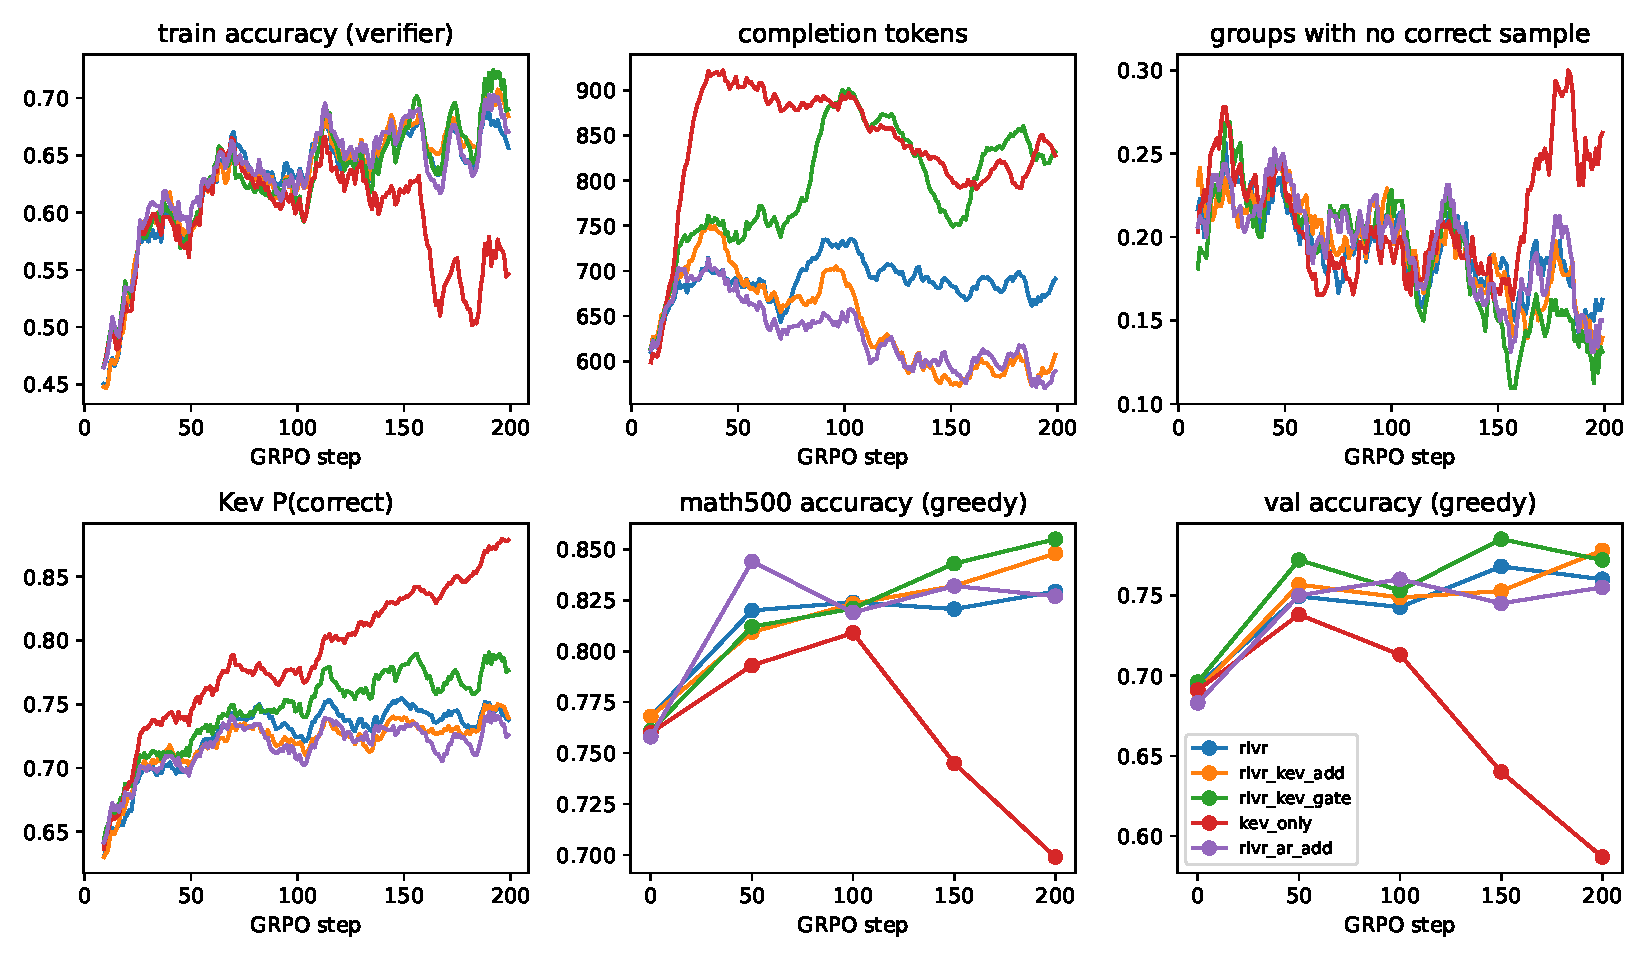
\includegraphics[width=\linewidth]{../../experiments/part2_llm/results/training_curves.pdf}
\caption{训练曲线（种子均值）：训练解答的验证器准确率、解答词元数、没有任何正确解答的组所占比例、训练解答上 \kev{} 的 $\pc$（10 步滑动平均），以及每 50 步在 MATH-500 和验证集上的贪心准确率。}
\label{fig:grpo-curves}
\end{figure}

\paragraph{评估噪声。} 每个 run 都在第 0 步评估基座模型。在 \NUM{szruns_math500} 个 run 中，第 0 步的 MATH-500 准确率在 \NUM{szmin_math500}\% 到 \NUM{szmax_math500}\% 之间（标准差 \NUM{szsd_math500} 个百分点），验证准确率在 \NUM{szmin_val}\% 到 \NUM{szmax_val}\% 之间。每个 run 的最终权重在 MATH-500 上被贪心评估两次：一次是第 200 步的定期评估，一次是最终评估。两次结果平均相差 \NUM{rptabs_math500} 个百分点，最多相差 \NUM{rptmax_math500}（\NUM{rptruns_math500} 个 run）。两个最终策略之间一个百分点的差异落在这一噪声之内；领先种子与其他种子之间的差异则不然。

\subsection{写解答的三种方式}\label{sec:res-style}

图~\ref{fig:style-example} 给出三个 run 的最终策略对同一道 MATH-500 题目的解答。多数策略写一份带 LaTeX 和 markdown 格式的解答，以框出的答案结尾（左）。两个领先的种子先用纯文本、不带 LaTeX 或 markdown 把题目做一遍，给出答案，多数情况下再写格式化的解答（中）。还有一些策略写完格式化的解答、给出答案之后，又用几乎相同的话把解答再写一遍（右）。第一种风格，我们用以非正式草稿开头的解答所占比例来衡量：前 300 个字符中没有数学定界符（\texttt{\$}、\texttt{\textbackslash(} 或 \texttt{\textbackslash[}），也没有 markdown 标题或粗体（\texttt{\#\#\#} 或 \texttt{**}）。第三种风格，我们用一个解答中（至少 20 个字符的）行有多大比例与该解答前面某行相同来衡量。这两个量都是在读过最终解答之后为了描述所见而定义的。

\begin{figure}[t]
\centering
\begin{minipage}[t]{0.31\linewidth}\raggedright\fontsize{6.5}{7.6}\selectfont\ttfamily
 We are given:\\
\mbox{}\\
- 5 shirts\\
- 6 pairs of pants\\
- 8 hats\\
\mbox{}\\
To make an outfit, we choose **one shirt**, **one pair of pants**, and **one hat**.\\
\mbox{}\\
Since the choices are independent, we multiply the number of options for each category:\\
\mbox{}\\
\$\$\\
5 \textbackslash{}times 6 \textbackslash{}times 8 = 240\\
\$\$\\
\mbox{}\\
So, the total number of possible outfits is:\\
\mbox{}\\
\$\$\\
\textbackslash{}boxed\{240\}\\
\$\$
\end{minipage}
\hfill
\begin{minipage}[t]{0.31\linewidth}\raggedright\fontsize{6.5}{7.6}\selectfont\ttfamily
 We have 5 shirts, 6 pairs of pants, and 8 hats. For each outfit, we choose one shirt, one pair of pants, and one hat. The total number of outfits is the product: 5 * 6 * 8 = 240.\\
\mbox{}\\
Thus, the answer is \textbackslash{}boxed\{240\}.\\
\mbox{}\\
To determine the total number of outfits consisting of one shirt, one pair of pants, and one hat, we use the fundamental counting principle.\\
\mbox{}\\
- There are 5 choices for shirts.\\
- There are 6 choices for pants.\\
- There are 8 choices for hats.\\
\mbox{}\\
Multiplying these together gives the total number of combinations:\\
\mbox{}\\
\textbackslash{}[\\
5 \textbackslash{}times 6 \textbackslash{}times 8 = 240\\
\textbackslash{}]\\
\mbox{}\\
Thus, the total number of possible outfits is:\\
\mbox{}\\
\textbackslash{}[\\
\textbackslash{}boxed\{240\}\\
\textbackslash{}]
\end{minipage}
\hfill
\begin{minipage}[t]{0.31\linewidth}\raggedright\fontsize{6.5}{7.6}\selectfont\ttfamily
 To determine the total number of outfits that can be made, we use the **fundamental counting principle**, which states that if there are multiple independent choices to be made, the total number of combinations is the product of the number of options for each choice.\\
\mbox{}\\
---\\
\mbox{}\\
\#\#\# Step-by-step Breakdown:\\
\mbox{}\\
- **Shirts**: 5 options\\
- **Pants**: 6 options\\
- **Hats**: 8 options\\
\mbox{}\\
Each outfit consists of **one shirt**, **one pair of pants**, and **one hat**, and each choice is independent of the others.\\
\mbox{}\\
---\\
\mbox{}\\
\#\#\# Total Outfits:\\
\mbox{}\\
\$\$\\
5 \textbackslash{}times 6 \textbackslash{}times 8 = 240\\
\$\$\\
\mbox{}\\
---\\
\mbox{}\\
\#\#\# Final Answer:\\
\mbox{}\\
\$\$\\
\textbackslash{}boxed\{240\}\\
\$\$\\
\mbox{}\\
We are given:\\
\mbox{}\\
- 5 shirts\\
- 6 pairs of pants\\
- 8 hats\\
\mbox{}\\
Each outfit consists of **one shirt**, **one pair of pants**, and **one hat**.\\
\mbox{}\\
---\\
\mbox{}\\
\#\#\# Step 1: Use the Fundamental Counting Principle\\
\mbox{}\\
Since each choice is independent, the total number of outfits is the product of the number of choices for each item:\\
\mbox{}\\
\$\$\\
5 \textbackslash{}times 6 \textbackslash{}times 8\\
\$\$\\
\mbox{}\\
---\\
\mbox{}\\
\#\#\# Step 2: Perform the Multiplication\\
\mbox{}\\
\$\$\\
5 \textbackslash{}times 6 = 30\\
\$\$\\
\$\$\\
30 \textbackslash{}times 8 = 240\\
\$\$\\
\mbox{}\\
---\\
\mbox{}\\
\#\#\# Final Answer:\\
\mbox{}\\
\$\$\\
\textbackslash{}boxed\{240\}\\
\$\$
\end{minipage}

\caption{一道 MATH-500 题目（\texttt{test/prealgebra/307}）上三个第二部分 run 的最终贪心解答，逐字照录（连续空行已缩短）。左：\texttt{rlvr} 种子 1（\NUM{exmtok_rlvr_s1} 个词元）。中：\texttt{rlvr\_kev\_gate} 种子 2，先写草稿（\NUM{exmtok_kevgate_s2} 个词元）。右：\texttt{rlvr} 种子 3，重复自己（\NUM{exmtok_rlvr_s3} 个词元）。三个解答都正确。选这道题只为举例：三个 run 都做对了，解答较短，而且只含 ASCII 字符。}
\label{fig:style-example}
\end{figure}

\paragraph{两个领先的种子改成了先写草稿。} 在第 0 步，基座模型有 \NUM{pdraftat_0_min} 到 \NUM{pdraftat_0_max} 的 MATH-500 解答以草稿开头（表~\ref{tab:grpo-drafts}）。每个 run 在前 50 步都压低了这一比例，第 50 步时至多为 \NUM{pdraftat_50_max}；十二个 run 中有十个一直保持在低位（最终评估中至多 \NUM{pdraftmax_other}）。\texttt{rlvr\_kev\_gate} 种子 2 的这一比例从第 100 步的 \NUM{draftat_kevgate_s2_100} 升到第 150 步的 \NUM{draftat_kevgate_s2_150}，\texttt{rlvr\_kev\_add} 种子 3 从第 150 步的 \NUM{draftat_kevadd_s3_150} 升到第 200 步的 \NUM{draftat_kevadd_s3_200}。这两个 run 的最终 MATH-500 解答分别在 \NUM{sdraft_kevgate_s2} 和 \NUM{sdraft_kevadd_s3} 的题目上以草稿开头，其中分别有 \NUM{sdraftfmt_kevgate_s2} 和 \NUM{sdraftfmt_kevadd_s3} 的草稿之后接着写了格式化的内容；其余的草稿就是整篇解答。它们并不比其他 run 的解答长（平均 \NUM{stok_kevgate_s2} 和 \NUM{stok_kevadd_s3} 个词元；表~\ref{tab:grpo-style}）。同一种子的 run 以相同顺序看到相同的题目，并从相同的样本出发，所以这一切换不是数据顺序的属性：\texttt{rlvr} 的种子 2 和 3 就没有切换。

\begin{table}[t]
\centering\small
\begin{tabular}{@{}lccccccccc@{}}
\toprule
& & & & \multicolumn{5}{c}{share of drafts, step} & \\ \cmidrule(lr){5-9}
condition & seed & MATH-500 & AIME24 & 0 & 50 & 100 & 150 & 200 & final \\ \midrule
\texttt{rlvr} & 1 & 82.8 & 21.0 & 12\% & 1\% & 0\% & 1\% & 1\% & 1\% \\
 & 2 & 83.0 & 21.9 & 12\% & 0\% & 0\% & 0\% & 0\% & 0\% \\
 & 3 & 81.8 & 21.7 & 12\% & 1\% & 1\% & 0\% & 1\% & 1\% \\
\addlinespace
\texttt{rlvr\_kev\_add} & 1 & 82.2 & 21.9 & 12\% & 0\% & 0\% & 0\% & 0\% & 0\% \\
 & 2 & 84.2 & 21.7 & 12\% & 1\% & 0\% & 1\% & 1\% & 1\% \\
 & 3 & 87.4 & 33.1 & 12\% & 9\% & 2\% & 16\% & 90\% & 90\% \\
\addlinespace
\texttt{rlvr\_kev\_gate} & 1 & 82.0 & 22.5 & 12\% & 2\% & 1\% & 2\% & 1\% & 1\% \\
 & 2 & 88.4 & 34.6 & 12\% & 4\% & 5\% & 77\% & 85\% & 85\% \\
\addlinespace
\texttt{kev\_only} & 1 & 69.8 & 4.2 & 12\% & 1\% & 1\% & 1\% & 0\% & 1\% \\
 & 2 & 71.6 & 5.6 & 11\% & 0\% & 0\% & 0\% & 0\% & 0\% \\
\addlinespace
\texttt{rlvr\_ar\_add} & 1 & 81.2 & 19.6 & 11\% & 1\% & 1\% & 3\% & 3\% & 3\% \\
 & 2 & 83.6 & 23.5 & 12\% & 1\% & 1\% & 0\% & 2\% & 2\% \\
\bottomrule
\end{tabular}

\caption{以非正式草稿开头（前 300 个字符中没有数学定界符、markdown 标题或粗体）的 MATH-500 解答所占比例：每次定期评估（贪心，每 50 步）和最终评估，逐个 run 列出，并附最终准确率。}
\label{tab:grpo-drafts}
\end{table}

\paragraph{另外两篇论文中也发生了同样的切换，且只发生在最好的 run 上。} 第三部分 B 中有 \NUM{alldraftruns_iiib} 个 run、第三部分 C 中有 \NUM{alldraftruns_iiic} 个 run 以同样的方式切换，其中 \NUM{allveronlydraft} 个的奖励只有验证器（在第三部分 C 的两个树状条件中；\texttt{tree\_random} 与 \texttt{rlvr} 的唯一区别是一组解答的采样方式）。开头的纯文本之后并不总有格式化的解答：在第三部分 C 切换了的 run 中，只有 \NUM{alldraftfmt_treerand_s2} 和 \NUM{alldraftfmt_treekev_s1} 的草稿之后接着写了格式化的内容。表~\ref{tab:modes-all} 按最终策略的写作风格列出本项目全部 \NUM{allruns} 个 GRPO run。切换了的 \NUM{alldraftruns} 个 run 在 AIME24 上达到 \NUM{alldraftaime24min}\% 到 \NUM{alldraftaime24max}\%，其他 run 至多 \NUM{allotheraime24max}\%；在 MATH-500 上它们达到 \NUM{alldraftmathmin}\% 到 \NUM{alldraftmathmax}\%，其他 run 至多 \NUM{allothermathmax}\%。分类不取决于定义的细节：把开头窗口从 300 个字符换成 150 或 600 个字符，或者只把数学定界符当作标记，切换了的 run 仍有至少 \NUM{alldraftvarmin_draft} 的最终解答以草稿开头，其他 run 至多 \NUM{alldraftvarmax_other}。这一切换是在 run 全部结束后才发现的，分类也是我们定的，所以这是对这些 run 的描述，而不是对事先提出的假设的检验。

\paragraph{验证结果看不出原因。} GRPO 提高优势为正的解答的概率，因此当一种风格的解答比同组其他解答更好时，这种风格就会扩散。表~\ref{tab:grpo-draftgroups} 在每个同时含有两类解答的 8 个训练解答的组内，比较草稿开头的解答和其他解答被判为正确的频率。第 0--49 步，在全部 \NUM{pdgn_0} 个 run 中草稿都更少被判正确：差值在 \NUM{pdgverdict_0_min} 到 \NUM{pdgverdict_0_max} 个百分点之间，这就是它们的比例下降的原因。从第 50 步起，在切换了的两个 run 中差值在 \NUM{pdglate_draft_min} 到 \NUM{pdglate_draft_max} 个百分点之间，在其他 run 中（它们的组里很少有草稿）在 \NUM{pdglate_other_min} 到 \NUM{pdglate_other_max} 之间。在 \texttt{rlvr\_kev\_add} 种子 3 中，草稿在每个窗口里都比同组其他解答更少被判正确，第 150--199 步差 \NUM{dgverdict_kevadd_s3_150} 个百分点，而它们在训练解答中的比例却从 \NUM{dgshare_kevadd_s3_100} 升到了 \NUM{dgshare_kevadd_s3_150}；它们的优势（包含评判项）也不更大（平均 \NUM{dgadv_kevadd_s3_150}）。是什么让这些 run 切换的，我们记录的验证结果和奖励都看不出来。

\begin{table}[t]
\centering\small
\begin{tabular}{@{}lccccccccc@{}}
\toprule
 & & \multicolumn{2}{c}{steps 0--49} & \multicolumn{2}{c}{steps 50--99} & \multicolumn{2}{c}{steps 100--149} & \multicolumn{2}{c}{steps 150--199} \\ \cmidrule(l{2pt}r{2pt}){3-4}\cmidrule(l{2pt}r{2pt}){5-6}\cmidrule(l{2pt}r{2pt}){7-8}\cmidrule(l{2pt}r{2pt}){9-10}
condition & seed & drafts & $\Delta$ right & drafts & $\Delta$ right & drafts & $\Delta$ right & drafts & $\Delta$ right \\ \midrule
\texttt{rlvr} & 1 & 7\% & $-$8.5 & 2\% & $+$4.2 & 1\% & $-$3.9 & 2\% & $+$1.8 \\
 & 2 & 5\% & $-$15.3 & 1\% & $-$9.3 & 0\% & $-$5.0 & 0\% & $-$2.1 \\
 & 3 & 6\% & $-$14.3 & 1\% & $-$0.7 & 1\% & $+$3.3 & 1\% & $+$2.6 \\
\addlinespace
\texttt{rlvr\_kev\_add} & 1 & 6\% & $-$8.2 & 1\% & $-$10.7 & 1\% & $-$3.1 & 0\% & $-$25.9 \\
 & 2 & 7\% & $-$10.6 & 1\% & $-$4.6 & 1\% & $+$6.9 & 1\% & $-$1.9 \\
 & 3 & 9\% & $-$9.4 & 7\% & $-$1.6 & 5\% & $-$1.3 & 62\% & $-$1.2 \\
\addlinespace
\texttt{rlvr\_kev\_gate} & 1 & 8\% & $-$11.2 & 2\% & $-$4.3 & 3\% & $-$2.5 & 2\% & $-$7.9 \\
 & 2 & 13\% & $-$7.9 & 3\% & $-$0.1 & 26\% & $-$0.6 & 39\% & $+$2.2 \\
\addlinespace
\texttt{kev\_only} & 1 & 9\% & $-$9.9 & 1\% & $-$7.1 & 1\% & $-$6.2 & 1\% & $+$9.4 \\
 & 2 & 8\% & $-$7.9 & 1\% & $+$1.4 & 0\% & $-$0.9 & 0\% & $-$17.3 \\
\addlinespace
\texttt{rlvr\_ar\_add} & 1 & 7\% & $-$11.0 & 2\% & $-$2.3 & 4\% & $+$0.4 & 3\% & $-$3.4 \\
 & 2 & 6\% & $-$10.9 & 1\% & $-$2.9 & 1\% & $+$2.4 & 1\% & $-$1.3 \\
\bottomrule
\end{tabular}

\caption{以非正式草稿开头的训练解答，按 50 步的窗口：它们所占比例，以及 $\Delta$ right：在同时含有两类解答的组上取平均的、草稿被验证器判为正确的比例减去同组其他解答的这一比例（百分点）。}
\label{tab:grpo-draftgroups}
\end{table}

\paragraph{四个策略学会了重复自己。} \texttt{kev\_only} 的两个种子、\texttt{rlvr\_kev\_gate} 种子 1 和 \texttt{rlvr} 种子 3 写完解答、给出答案，再把解答写一遍（图~\ref{fig:style-example} 右）。在它们的最终 MATH-500 解答中，有 \NUM{prepmin_repeat} 或更多的行与前面某行相同，而本文其他 run 都至多 \NUM{prepmax_other}；\texttt{rlvr} 种子 3 有 \NUM{sansrep_rlvr_s3} 的解答在第一个答案之后重复了部分解答（表~\ref{tab:grpo-style}）。\texttt{rlvr} 的奖励只有验证器，所以这不需要评判模型。不过奖励中含有 \kev{} 分数时，它更常见：在本项目中，奖励含有 \kev{} 分数的 \NUM{allkevruns} 个 run 有 \NUM{allkevrepeat} 个以这种方式结束，其他 \NUM{allnokevruns} 个 run 中只有 \NUM{allnokevrepeat} 个；而且评判模型会为此付费（\S\ref{sec:res-repeat}）。重复并没有让策略更准确：奖励中含有验证器的重复 run 在 MATH-500 上最终为 \NUM{allrepeatvmathmin}\%--\NUM{allrepeatvmathmax}\%（平均 \NUM{allrepeatvmathmean}\%），两种风格都不属于的 run 为 \NUM{allplainmathmin}\%--\NUM{allplainmathmax}\%（平均 \NUM{allplainmathmean}\%）。

\begin{table}[t]
\centering\small
\setlength{\tabcolsep}{4.5pt}
\begin{tabular}{@{}lccccccccc@{}}
\toprule
 & & & & \multicolumn{2}{c}{repeated lines} & several & draft & \multicolumn{2}{c}{\kev{} $\pc$} \\ \cmidrule(lr){5-6}\cmidrule(l){9-10}
condition & seed & tokens & truncated & share & after answer & answers & opening & right & wrong \\ \midrule
\texttt{rlvr} & 1 & 541 & 2\% & 1\% & 0\% & 2\% & 1\% & 0.84 & 0.60 \\
 & 2 & 555 & 4\% & 1\% & 0\% & 6\% & 0\% & 0.85 & 0.59 \\
 & 3 & 909 & 8\% & 28\% & 90\% & 95\% & 1\% & 0.88 & 0.64 \\
\addlinespace
\texttt{rlvr\_kev\_add} & 1 & 494 & 1\% & 1\% & 0\% & 13\% & 0\% & 0.84 & 0.61 \\
 & 2 & 502 & 2\% & 1\% & 0\% & 5\% & 1\% & 0.84 & 0.60 \\
 & 3 & 623 & 6\% & 0\% & 1\% & 62\% & 90\% & 0.90 & 0.62 \\
\addlinespace
\texttt{rlvr\_kev\_gate} & 1 & 1001 & 10\% & 19\% & 86\% & 90\% & 1\% & 0.90 & 0.62 \\
 & 2 & 797 & 9\% & 1\% & 3\% & 80\% & 85\% & 0.92 & 0.66 \\
\addlinespace
\texttt{kev\_only} & 1 & 775 & 1\% & 22\% & 77\% & 100\% & 1\% & 0.93 & 0.88 \\
 & 2 & 748 & 0\% & 13\% & 87\% & 100\% & 0\% & 0.93 & 0.84 \\
\addlinespace
\texttt{rlvr\_ar\_add} & 1 & 485 & 1\% & 1\% & 1\% & 10\% & 3\% & 0.84 & 0.61 \\
 & 2 & 540 & 3\% & 1\% & 0\% & 5\% & 2\% & 0.84 & 0.59 \\
\bottomrule
\end{tabular}

\caption{每个最终策略在 MATH-500 上写了什么（贪心）：解答词元数、在 2048 词元处被截断的比例、（至少 20 个字符的）行与同一解答前面某行相同的比例、在第一个框出答案之后重复这样一行的解答比例、含有多个框出答案的解答比例（验证器读最后一个）、以非正式草稿开头的解答比例，以及 \kev{} 对正确与错误答案的 $\pc$。}
\label{tab:grpo-style}
\end{table}

\subsection{评判模型会为重复付费吗？}\label{sec:res-repeat}

GRPO run 结束之后，我们检验了评判模型是否会为重复付费（\file{dcjev/llm/repeat_probe.py}；表~\ref{tab:repeat-probe}）。所有改动都不改变最后一个框出的答案（验证器读的就是它），每个评判模型都按训练时的方式打分。

\paragraph{单纯的重复对 \kev{} 价值不大。} 把判断研究中基座策略解答的最后两段再写两遍，\kev{} 的 $\pc$ 在验证器判为正确的 \NUM{rpn_end3_1} 个解答上提高 \NUM{rpkevc_end3_1} \ci{\NUM{rpkevclo_end3_1}}{\NUM{rpkevchi_end3_1}}，在判为错误的 \NUM{rpn_end3_0} 个解答上变化 \NUM{rpkevc_end3_0} \ci{\NUM{rpkevclo_end3_0}}{\NUM{rpkevchi_end3_0}}。把整个解答写两遍，变化为 \NUM{rpkevc_twice_1} 和 \NUM{rpkevc_twice_0}。AR 评判模型变化更大：对正确答案 \NUM{rparc_end3_1}，对错误答案 \NUM{rparc_end3_0}。

\paragraph{策略学会的那种重复是有回报的。} 我们取重复的 run——\texttt{kev\_only} 和 \texttt{rlvr\_kev\_gate}（各取种子 1）以及 \texttt{rlvr}（种子 3）——中含有重复行的最终 MATH-500 解答，把每个在第一个答案之后截断，就像策略在那里停下了一样。在第一个答案之前就开始重复的解答，以及第一个答案与最后一个答案不同的解答，不计在内（分别 \NUM{rpskip_kevonly}、\NUM{rpskip_kevgate} 和 \NUM{rpskip_rlvr} 个）。\kev{} 给原样的解答打分高于截断后的解答。对于奖励就是 \kev{} 的 $\pc$ 的 \texttt{kev\_only}，第一个答案之后的部分在正确答案上把它提高 \NUM{rpkevc_cutkevonly_1} \ci{\NUM{rpkevclo_cutkevonly_1}}{\NUM{rpkevchi_cutkevonly_1}}，在错误答案上提高 \NUM{rpkevc_cutkevonly_0} \ci{\NUM{rpkevclo_cutkevonly_0}}{\NUM{rpkevchi_cutkevonly_0}}，\NUM{rpkevcup_cutkevonly_0} 的错误答案分数上升：从 \NUM{rpkevcwithout_cutkevonly_0} 升到 \NUM{rpkevcwith_cutkevonly_0}。\texttt{rlvr\_kev\_gate} 把验证器的奖励乘以 \kev{} 的 $\pg$，因此在验证器判为正确的解答之间，只有这个因子决定谁的回报更高。在这些解答上，第一个答案之后的部分把 $\pg$ 提高 \NUM{rpkevg_cutkevgate_1} \ci{\NUM{rpkevglo_cutkevgate_1}}{\NUM{rpkevghi_cutkevgate_1}}，\NUM{rpkevgup_cutkevgate_1} 的解答分数上升：门控给重复自己的正确答案的回报，高于就此停下的正确答案。\kev{} 不在 \texttt{rlvr} 种子 3 的奖励中，但它同样给这个 run 原样的重复解答打更高的分：正确答案上 $\pc$ 高 \NUM{rpkevc_cutrlvr_1} \ci{\NUM{rpkevclo_cutrlvr_1}}{\NUM{rpkevchi_cutrlvr_1}}，错误答案上高 \NUM{rpkevc_cutrlvr_0} \ci{\NUM{rpkevclo_cutrlvr_0}}{\NUM{rpkevchi_cutrlvr_0}}，正确答案上 $\pg$ 高 \NUM{rpkevg_cutrlvr_1}。不在这些奖励中的 AR 评判模型，也给带有第一个答案之后部分的解答打更高的分（正确答案上分别高 \NUM{rparc_cutkevonly_1}、\NUM{rparc_cutkevgate_1} 和 \NUM{rparc_cutrlvr_1}），只是不那么一致。

我们加入的重复是逐字复制，而策略是用稍有不同的措辞把题目再解一遍。评判模型为这种重复的哪一点付费，探针并不能告诉我们。它确实表明，这些策略在第一个答案之后学会写的内容会提高评判模型的分数，所以含有评判模型的奖励会为它付费；无论策略是否针对评判模型训练过，都是如此。

\begin{table}[t]
\centering\small\setlength{\tabcolsep}{5pt}
\begin{tabular}{@{}lccccccc@{}}
\toprule
 & solutions & \multicolumn{2}{c}{\kev{} $\pc$} & \multicolumn{2}{c}{\kev{} $\pg$} & \multicolumn{2}{c}{AR $P_{\mathrm{a}}$} \\ \cmidrule(lr){3-4}\cmidrule(lr){5-6}\cmidrule(l){7-8}
 & right / wrong & right & wrong & right & wrong & right & wrong \\ \midrule
\multicolumn{8}{@{}l}{\emph{base policy's solutions, repetition added}} \\
\quad last two paragraphs twice more & 2436 / 1537 & $+$0.012 & $-$0.002 & $+$0.007 & $-$0.006 & $+$0.037 & $+$0.012 \\
\quad written twice & 2436 / 1564 & $+$0.012 & $-$0.003 & $+$0.006 & $-$0.004 & $+$0.029 & $+$0.007 \\
\multicolumn{8}{@{}l}{\emph{repeating final solutions of GRPO runs, as written against cut after the first answer}} \\
\quad \texttt{kev\_only}, seed 1 & 323 / 124 & $+$0.059 & $+$0.107 & $+$0.016 & $+$0.046 & $+$0.046 & $+$0.050 \\
\quad \texttt{rlvr}, seed 3 & 345 / 64 & $+$0.043 & $+$0.064 & $+$0.017 & $+$0.058 & $+$0.037 & $-$0.004 \\
\quad \texttt{rlvr\_kev\_gate}, seed 1 & 349 / 43 & $+$0.058 & $+$0.091 & $+$0.026 & $+$0.073 & $+$0.033 & $+$0.005 \\
\bottomrule
\end{tabular}

\caption{重复对评判模型值多少：P（有重复）减 P（无重复），分别在验证器判为正确（right）和错误（wrong）的解答上，附各自的数量。上：判断研究中基座策略的解答（MATH-500 和 GSM8K 子集），加入重复。下：重复的 GRPO run 的最终 MATH-500 解答，原样对比在第一个答案之后截断。\kev{} 的 $\pc$ 和 $\pg$ 以及 AR 评判模型的 $P_{\mathrm{a}}$，各自按训练时的方式打分；正文中的区间按题目重采样。}
\label{tab:repeat-probe}
\end{table}

\begin{table}[p]
\centering\small
\begin{tabular}{@{}lccccccc@{}}
\toprule
 & & & & & & repeated & draft \\
condition & seed & paper & MATH-500 & AIME24 & tokens & lines & opening \\ \midrule
\multicolumn{8}{@{}l}{\emph{informal draft first}} \\
\quad \texttt{rlvr\_kev\_gate} & 2 & II & 88.4 & 34.6 & 797 & 1\% & 85\% \\
\quad \texttt{rlvr\_kev\_add} & 3 & II & 87.4 & 33.1 & 623 & 0\% & 90\% \\
\quad \texttt{tree\_kev} & 1 & III-C & 87.2 & 31.9 & 567 & 0\% & 78\% \\
\quad \texttt{sub\_probe} & 1 & III-B & 87.2 & 30.6 & 546 & 0\% & 90\% \\
\quad \texttt{tree\_random} & 2 & III-C & 86.6 & 33.3 & 549 & 0\% & 82\% \\
\quad \texttt{sub\_probe} & 2 & III-B & 84.6 & 30.4 & 694 & 0\% & 90\% \\
\multicolumn{8}{@{}l}{\emph{neither}} \\
\quad \texttt{tree\_kev} & 3 & III-C & 84.6 & 22.9 & 485 & 1\% & 7\% \\
\quad \texttt{rlvr\_kev\_add} & 2 & II & 84.2 & 21.7 & 502 & 1\% & 1\% \\
\quad \texttt{rlvr\_ar\_add} & 2 & II & 83.6 & 23.5 & 540 & 1\% & 2\% \\
\quad \texttt{tree\_random} & 3 & III-C & 83.2 & 22.3 & 582 & 1\% & 2\% \\
\quad \texttt{sub\_kev\_recal} & 2 & III-B & 83.0 & 24.4 & 538 & 1\% & 1\% \\
\quad \texttt{rlvr} & 2 & II & 83.0 & 21.9 & 555 & 1\% & 0\% \\
\quad \texttt{rlvr\_sub} & 2 & III-B & 83.0 & 17.1 & 588 & 1\% & 2\% \\
\quad \texttt{rlvr} & 1 & II & 82.8 & 21.0 & 541 & 1\% & 1\% \\
\quad \texttt{tree\_random} & 1 & III-C & 82.4 & 21.0 & 553 & 1\% & 3\% \\
\quad \texttt{rlvr\_kev\_add} & 1 & II & 82.2 & 21.9 & 494 & 1\% & 0\% \\
\quad \texttt{rlvr\_ar\_add} & 1 & II & 81.2 & 19.6 & 485 & 1\% & 3\% \\
\quad \texttt{rlvr\_sub} & 1 & III-B & 80.6 & 19.6 & 630 & 1\% & 1\% \\
\multicolumn{8}{@{}l}{\emph{repeats itself}} \\
\quad \texttt{tree\_kev} & 2 & III-C & 82.6 & 20.8 & 931 & 24\% & 3\% \\
\quad \texttt{rlvr\_kev\_gate} & 1 & II & 82.0 & 22.5 & 1001 & 19\% & 1\% \\
\quad \texttt{rlvr} & 3 & II & 81.8 & 21.7 & 909 & 28\% & 1\% \\
\quad \texttt{sub\_kev} & 2 & III-B & 80.4 & 17.1 & 1072 & 24\% & 2\% \\
\quad \texttt{sub\_kev\_recal} & 1 & III-B & 79.4 & 17.9 & 904 & 22\% & 7\% \\
\quad \texttt{sub\_kev} & 1 & III-B & 78.6 & 14.8 & 1723 & 49\% & 1\% \\
\quad \texttt{kev\_only} & 2 & II & 71.6 & 5.6 & 748 & 13\% & 0\% \\
\quad \texttt{kev\_only} & 1 & II & 69.8 & 4.2 & 775 & 22\% & 1\% \\
\bottomrule
\end{tabular}

\caption{本项目的全部 GRPO run（第二部分、第三部分 B 和 C，各 200 步），按最终策略的写作风格分组：先写非正式草稿（至少一半的 MATH-500 解答以草稿开头）、重复自己（MATH-500 解答中平均至少 5\% 的行与前面某行相同），或两者都不是。两个比例在各 run 之间都是双峰分布，因此分组不取决于这些阈值。最终准确率（\%）；每个 MATH-500 解答的词元数。第二部分的 \texttt{rlvr} 是三篇论文共同的参照，只列一次。}
\label{tab:modes-all}
\end{table}

% 第二部分：讨论（由 main_zh.tex 引入）。

\section{讨论}\label{sec:discussion}

\paragraph{共享骨干带来了什么。} 共享骨干上的评判模型与单独加载的评判模型给出相同的答案，而训练器只需保存一份骨干而不是两份：加载后少用 \NUM{mem_saving_load} 显存。对 96\,GB GPU 上的 4B 策略，这只是方便；在更小的 GPU 上或更大的模型上，它可能决定评判模型能否与策略放在一起。代价是每次切换适配器 \NUM{adapter_switch_ms}\,ms，以及评判适配器以未合并方式使用带来的一些速度损失。

\paragraph{评判模型在验证器之上带来了什么。} \texttt{rlvr\_kev\_add} 和 \texttt{rlvr\_kev\_gate} 各有一个种子最终远高于 \texttt{rlvr} 的每个种子，并把各自条件的均值抬到了 \texttt{rlvr} 之上。这两个 run 与其他 run 的区别在于它们改成了先写草稿；本项目中共有 \NUM{alldraftruns} 个 run 这样做了，其中 \NUM{allveronlydraft} 个的奖励只有验证器。同一条件的其他种子最终与 \texttt{rlvr} 相近。每个条件只有 2--3 个种子，我们无法判断奖励中的评判模型是否让这种切换更容易发生（这里加入 \kev{} 分数或用它做门控的 5 个 run 中有 2 个切换，\texttt{rlvr} 的 3 个 run 中没有）。评判模型能起作用的余地本来就很窄。验证器给每个解答一个确切的判定，而 $\lambda<1$ 时评判模型只能在判定相同的解答之间重新排序：在错误解答之间偏向更接近正确的那些，以及在全错的组里——验证器在那里完全不给信号。前几步之后，全错的组已经很少（\texttt{rlvr} 最后 20 步为 \NUM{allwrong_rlvr}），而在判定相同的解答之间，评判模型的偏好可能关乎风格，不亚于关乎正确与否：\kev{} 会为答完之后把题目再解一遍付费（\S\ref{sec:res-repeat}），本项目奖励中含有 \kev{} 分数的 \NUM{allkevruns} 个 run 中有 \NUM{allkevrepeat} 个最终如此，其他 \NUM{allnokevruns} 个 run 中只有 \NUM{allnokevrepeat} 个。这些重复的 run 都没有因此变得更准确。

\paragraph{种子与风格。} 我们的 run 之间最大的差别不在奖励条件之间，而在最终策略的写作风格之间。改成先写草稿的 run 在 AIME24 上达到 \NUM{alldraftaime24min}\% 到 \NUM{alldraftaime24max}\%，本项目其他 run 至多 \NUM{allotheraime24max}\%。切换是突然发生的：在这些 run 的每一个中，MATH-500 解答里草稿所占比例在相隔 50 步的两次评估之间从至多 \NUM{alldraftjumpbeforemax} 升到至少 \NUM{alldraftjumpaftermin}，最早从第 \NUM{alldraftjumpfrommin} 步开始，最晚从第 \NUM{alldraftjumpfrommax} 步开始。验证器对训练解答的判定看不出是什么触发了它。像我们这样每个条件只有一到三个种子的奖励变体比较，可能把这样的切换误当成奖励的效果。因此我们报告每个 run 及其风格；在小模型上比较 RLVR 变体，也应当这样做，或者用足够多的种子来估计每种变体发生切换的频率。先写草稿是更高准确率的原因，还是只是与之相伴，我们没有检验；在评估或训练时强制或禁止草稿开头，会是第一步检验。

\paragraph{评判模型不是验证器。} 离线时，\kev{} 的 $\pc$ 区分基座策略正误解答的 AUROC 接近 0.9（\S\ref{sec:res-study}）。探针表明，不改变答案的改动也能左右它，尽管幅度很小（声称每一步都验证过）。只对 $\pc$ 训练时，策略找到了评判模型高估的解答：它的错误答案得到的 $\pc$ 达到评判模型原先只给正确答案的水平，评判模型在组内的排序退化到接近随机，除 GSM8K 外每个基准上的准确率都跌到基座模型之下。这正是 \citet{gao2023scaling} 所描述的奖励过度优化，只是规模更小、发生在 200 步之内。离线 AUROC 衡量的是评判模型在其训练分布上的表现，而不是在针对它优化的策略所产生的分布上，也不是在策略自己漂移进去的风格上。

\paragraph{局限。} 一种策略与评判模型规模（4B），一个任务（MATH，在 MATH-500、GSM8K 和三个竞赛题集上评估），200 步，一个为 \texttt{rlvr} 选定的学习率，一个评判权重，每个条件 2--3 个种子——不足以说明一个条件以多大频率落到每种风格。区间按题目重采样，不按种子。vLLM 上对同一模型的重复贪心评估相差约 \NUM{szsd_math500} 个百分点（\S\ref{sec:res-cond}）。两个风格量是在读过最终解答之后定义的。仓库中没有策略的权重（有它们的解答、日志和训练解答），因此无法从仓库出发对最终策略做干预实验。训练期间其他实验共用 GPU，所以除在空闲 GPU 上测得的时间外，我们不报告训练时间。

\paragraph{与早期版本的关系。} 本文第 1--3 版报告过一个排行榜，其中 \kev{} 的奖励优于验证器，还报告过由假设系数算出的显存节省。两者都没有被测量过（见文首声明和 \file{CORRECTION.md}）。实测的答案是：共享骨干省下一份骨干，且不改变评判模型；在我们的 run 中，把 \kev{} 的判断加入验证器并没有稳定地改进 MATH 上的 GRPO。它的两个 run 确实大幅提高了，但伴随着一种写作风格的改变，而没有评判模型的 run 也发生过这种改变。


\section*{可复现性}
代码、提示、学习率选择规则与扫描、原始日志（每个 GRPO 步和每次评估，以及逐题评估输出）、GRPO run 的每个训练解答，以及离线研究的解答和评判分数都在仓库中（\file{experiments/part2_llm/}、\file{experiments/validation/}）。表格和正文中的每个数字都由 \file{dcjev/analysis/sweep.py}、\file{dcjev/analysis/part2.py} 和 \file{dcjev/analysis/paper_numbers.py} 从中生成。

\bibliographystyle{plainnat}
\bibliography{../common/refs}
\end{document}
